% Options for packages loaded elsewhere
\PassOptionsToPackage{unicode}{hyperref}
\PassOptionsToPackage{hyphens}{url}
%
\documentclass[
]{book}
\usepackage{amsmath,amssymb}
\usepackage{lmodern}
\usepackage{ifxetex,ifluatex}
\ifnum 0\ifxetex 1\fi\ifluatex 1\fi=0 % if pdftex
  \usepackage[T1]{fontenc}
  \usepackage[utf8]{inputenc}
  \usepackage{textcomp} % provide euro and other symbols
\else % if luatex or xetex
  \usepackage{unicode-math}
  \defaultfontfeatures{Scale=MatchLowercase}
  \defaultfontfeatures[\rmfamily]{Ligatures=TeX,Scale=1}
\fi
% Use upquote if available, for straight quotes in verbatim environments
\IfFileExists{upquote.sty}{\usepackage{upquote}}{}
\IfFileExists{microtype.sty}{% use microtype if available
  \usepackage[]{microtype}
  \UseMicrotypeSet[protrusion]{basicmath} % disable protrusion for tt fonts
}{}
\makeatletter
\@ifundefined{KOMAClassName}{% if non-KOMA class
  \IfFileExists{parskip.sty}{%
    \usepackage{parskip}
  }{% else
    \setlength{\parindent}{0pt}
    \setlength{\parskip}{6pt plus 2pt minus 1pt}}
}{% if KOMA class
  \KOMAoptions{parskip=half}}
\makeatother
\usepackage{xcolor}
\IfFileExists{xurl.sty}{\usepackage{xurl}}{} % add URL line breaks if available
\IfFileExists{bookmark.sty}{\usepackage{bookmark}}{\usepackage{hyperref}}
\hypersetup{
  pdftitle={ml4ec - Machine Learning for Eddy Covariance data},
  pdfauthor={Benjamin Stocker},
  hidelinks,
  pdfcreator={LaTeX via pandoc}}
\urlstyle{same} % disable monospaced font for URLs
\usepackage{color}
\usepackage{fancyvrb}
\newcommand{\VerbBar}{|}
\newcommand{\VERB}{\Verb[commandchars=\\\{\}]}
\DefineVerbatimEnvironment{Highlighting}{Verbatim}{commandchars=\\\{\}}
% Add ',fontsize=\small' for more characters per line
\usepackage{framed}
\definecolor{shadecolor}{RGB}{248,248,248}
\newenvironment{Shaded}{\begin{snugshade}}{\end{snugshade}}
\newcommand{\AlertTok}[1]{\textcolor[rgb]{0.94,0.16,0.16}{#1}}
\newcommand{\AnnotationTok}[1]{\textcolor[rgb]{0.56,0.35,0.01}{\textbf{\textit{#1}}}}
\newcommand{\AttributeTok}[1]{\textcolor[rgb]{0.77,0.63,0.00}{#1}}
\newcommand{\BaseNTok}[1]{\textcolor[rgb]{0.00,0.00,0.81}{#1}}
\newcommand{\BuiltInTok}[1]{#1}
\newcommand{\CharTok}[1]{\textcolor[rgb]{0.31,0.60,0.02}{#1}}
\newcommand{\CommentTok}[1]{\textcolor[rgb]{0.56,0.35,0.01}{\textit{#1}}}
\newcommand{\CommentVarTok}[1]{\textcolor[rgb]{0.56,0.35,0.01}{\textbf{\textit{#1}}}}
\newcommand{\ConstantTok}[1]{\textcolor[rgb]{0.00,0.00,0.00}{#1}}
\newcommand{\ControlFlowTok}[1]{\textcolor[rgb]{0.13,0.29,0.53}{\textbf{#1}}}
\newcommand{\DataTypeTok}[1]{\textcolor[rgb]{0.13,0.29,0.53}{#1}}
\newcommand{\DecValTok}[1]{\textcolor[rgb]{0.00,0.00,0.81}{#1}}
\newcommand{\DocumentationTok}[1]{\textcolor[rgb]{0.56,0.35,0.01}{\textbf{\textit{#1}}}}
\newcommand{\ErrorTok}[1]{\textcolor[rgb]{0.64,0.00,0.00}{\textbf{#1}}}
\newcommand{\ExtensionTok}[1]{#1}
\newcommand{\FloatTok}[1]{\textcolor[rgb]{0.00,0.00,0.81}{#1}}
\newcommand{\FunctionTok}[1]{\textcolor[rgb]{0.00,0.00,0.00}{#1}}
\newcommand{\ImportTok}[1]{#1}
\newcommand{\InformationTok}[1]{\textcolor[rgb]{0.56,0.35,0.01}{\textbf{\textit{#1}}}}
\newcommand{\KeywordTok}[1]{\textcolor[rgb]{0.13,0.29,0.53}{\textbf{#1}}}
\newcommand{\NormalTok}[1]{#1}
\newcommand{\OperatorTok}[1]{\textcolor[rgb]{0.81,0.36,0.00}{\textbf{#1}}}
\newcommand{\OtherTok}[1]{\textcolor[rgb]{0.56,0.35,0.01}{#1}}
\newcommand{\PreprocessorTok}[1]{\textcolor[rgb]{0.56,0.35,0.01}{\textit{#1}}}
\newcommand{\RegionMarkerTok}[1]{#1}
\newcommand{\SpecialCharTok}[1]{\textcolor[rgb]{0.00,0.00,0.00}{#1}}
\newcommand{\SpecialStringTok}[1]{\textcolor[rgb]{0.31,0.60,0.02}{#1}}
\newcommand{\StringTok}[1]{\textcolor[rgb]{0.31,0.60,0.02}{#1}}
\newcommand{\VariableTok}[1]{\textcolor[rgb]{0.00,0.00,0.00}{#1}}
\newcommand{\VerbatimStringTok}[1]{\textcolor[rgb]{0.31,0.60,0.02}{#1}}
\newcommand{\WarningTok}[1]{\textcolor[rgb]{0.56,0.35,0.01}{\textbf{\textit{#1}}}}
\usepackage{longtable,booktabs,array}
\usepackage{calc} % for calculating minipage widths
% Correct order of tables after \paragraph or \subparagraph
\usepackage{etoolbox}
\makeatletter
\patchcmd\longtable{\par}{\if@noskipsec\mbox{}\fi\par}{}{}
\makeatother
% Allow footnotes in longtable head/foot
\IfFileExists{footnotehyper.sty}{\usepackage{footnotehyper}}{\usepackage{footnote}}
\makesavenoteenv{longtable}
\usepackage{graphicx}
\makeatletter
\def\maxwidth{\ifdim\Gin@nat@width>\linewidth\linewidth\else\Gin@nat@width\fi}
\def\maxheight{\ifdim\Gin@nat@height>\textheight\textheight\else\Gin@nat@height\fi}
\makeatother
% Scale images if necessary, so that they will not overflow the page
% margins by default, and it is still possible to overwrite the defaults
% using explicit options in \includegraphics[width, height, ...]{}
\setkeys{Gin}{width=\maxwidth,height=\maxheight,keepaspectratio}
% Set default figure placement to htbp
\makeatletter
\def\fps@figure{htbp}
\makeatother
\setlength{\emergencystretch}{3em} % prevent overfull lines
\providecommand{\tightlist}{%
  \setlength{\itemsep}{0pt}\setlength{\parskip}{0pt}}
\setcounter{secnumdepth}{5}
\usepackage{booktabs}
\ifluatex
  \usepackage{selnolig}  % disable illegal ligatures
\fi
\usepackage[]{natbib}
\bibliographystyle{apalike}

\title{ml4ec - Machine Learning for Eddy Covariance data}
\author{Benjamin Stocker}
\date{2021-09-02}

\begin{document}
\maketitle

{
\setcounter{tocdepth}{1}
\tableofcontents
}
\hypertarget{set-up}{%
\chapter{Set up}\label{set-up}}

\hypertarget{apps}{%
\section{Apps}\label{apps}}

For this workshop, you need \href{https://www.r-project.org/}{R} and \href{https://www.rstudio.com/products/rstudio/download/}{RStudio}. Follow the links for downloading and installing these apps.

\hypertarget{libraries}{%
\section{Libraries}\label{libraries}}

Install missing packages for this tutorial.

\begin{Shaded}
\begin{Highlighting}[]
\NormalTok{list\_pkgs }\OtherTok{\textless{}{-}} \FunctionTok{c}\NormalTok{(}\StringTok{"caret"}\NormalTok{, }\StringTok{"recipes"}\NormalTok{, }\StringTok{"rsample"}\NormalTok{, }\StringTok{"tidyverse"}\NormalTok{, }\StringTok{"conflicted"}\NormalTok{, }\StringTok{"modelr"}\NormalTok{, }\StringTok{"forcats"}\NormalTok{, }\StringTok{"yardstick"}\NormalTok{, }\StringTok{"visdat"}\NormalTok{, }\StringTok{"skimr"}\NormalTok{, }\StringTok{"ranger"}\NormalTok{, }\StringTok{"knitr"}\NormalTok{)}
\NormalTok{new\_pkgs }\OtherTok{\textless{}{-}}\NormalTok{ list\_pkgs[}\SpecialCharTok{!}\NormalTok{(list\_pkgs }\SpecialCharTok{\%in\%} \FunctionTok{installed.packages}\NormalTok{()[, }\StringTok{"Package"}\NormalTok{])]}
\ControlFlowTok{if}\NormalTok{ (}\FunctionTok{length}\NormalTok{(new\_pkgs) }\SpecialCharTok{\textgreater{}} \DecValTok{0}\NormalTok{) }\FunctionTok{install.packages}\NormalTok{(new\_pkgs)}
\end{Highlighting}
\end{Shaded}

This book was compiled with the \emph{bookdown} library and source files (RMarkdown), available on \href{https://github.com/stineb/ml4ec_workshop}{Github}. Navigate there also for working on the exercises (Chapter \ref{exercises}) and using the solutions (Chapter \ref{solutions}).

This book is published under a GNU-GPL v3 license. Please cite this as:

\emph{xxxx}

\hypertarget{introduction}{%
\chapter{Introduction}\label{introduction}}

\hypertarget{learning-objectives}{%
\section{Learning objectives}\label{learning-objectives}}

After this workshop unit, you will be able to \ldots{}

\begin{itemize}
\tightlist
\item
  Understand how overfitting models can happen and how it can be avoided.
\item
  Implement a typical workflow using a machine learning model for a supervised regression problem.
\item
  Evaluate the power of the model
\end{itemize}

\hypertarget{some-primers}{%
\section{Some primers}\label{some-primers}}

Machine learning (ML) refers to a class of algorithms that generate statistical models of data. There are two main types of machine learning:

\textbf{Unsupervised machine learning}: Detecting patterns without prior specification.

\textbf{Supervised machine learning}: Model fitting by optimising predictions for a given target.

\textbf{Loss} is a function predicted and observed values derived from the validation set. It is minimised during model training.

\hypertarget{overfitting}{%
\section{Overfitting}\label{overfitting}}

\emph{This example is based on \href{https://scikit-learn.org/stable/auto_examples/model_selection/plot_underfitting_overfitting.html}{this example from scikit-learn}.}

Machine learning (ML) may appear magical. The ability of ML algorithms to detect patterns and make predictions is fascinating. However, several challenges have to be met in the process of formulating, training, and evaluating the models. In this practical we will discuss some basics of supervised ML and how to achieve best predictive results.

In general, the aim of supervised ML is to find a model \(\hat{Y} = f(X)\) that is \emph{trained} (calibrated) using observed relationships between a set of \emph{features} (also known as \emph{predictors}, or \emph{labels}, or \emph{independent variables}) \(X\) and the \emph{target} variable \(Y\). Note, that \(Y\) is observed. The hat on \(\hat{Y}\) denotes an estimate. Some algorithms can even handle predictions of multiple target variables simultaneously (e.g., neural networks). ML algorithms consist of (more or less) flexible mathematical models with a certain structure and set of parameters. At the simple extreme end of the model spectrum is the univariate linear regression. You may not want to call this a ML algorithm because there is no iterative learning involved. Nevertheless, also univariate linear regression provides a prediction \(\hat{Y} = f(X)\), just like other (proper) ML algorithms do. The functional form of a linear regression is not particularly flexible (just a straight line for the best fit between predictors and targets) and it has only two parameters (slope and intercept). At the other extreme end are, for example, deep neural networks. They are extremely flexible, can learn highly non-linear relationships and deal with interactions between a large number of predictors. They also contain very large numbers of parameters, typically on the order of thousands. You can imagine that this allows these types of algorithms to very effectively learn from the data, but also bears the risk of \emph{overfitting}.

What is overfitting? The following example illustrates it. Let's assume that there is some true underlying relationship between a predictor \(x\) and the target variable \(y\). We don't know this relationship (in the code below, this is \texttt{true\_fun()}) and the observations contain a (normally distributed) error (\texttt{y\ =\ true\_fun(x)\ +\ 0.1\ *\ rnorm(n\_samples)}). Based on our training data (\texttt{df\_train}), we fit three polynomial models of degree 1, 4, and 15 to the observations. A polynomial of degree N is given by: \[
y = \sum_{n=0}^N a_n x^n
\] \(a_n\) are the coefficients, i.e., model parameters. The goal of the training is to get the coefficients \(a_n\). From the above definition, the polynomial of degree 15 has 16 parameters, while the polynomial of degree 1 has two parameters (and corresponds to a simple linear regression). You can imagine that the polynomial of degree 15 is much more flexible and should thus yield the closest fit to the training data. This is indeed the case.

\begin{center}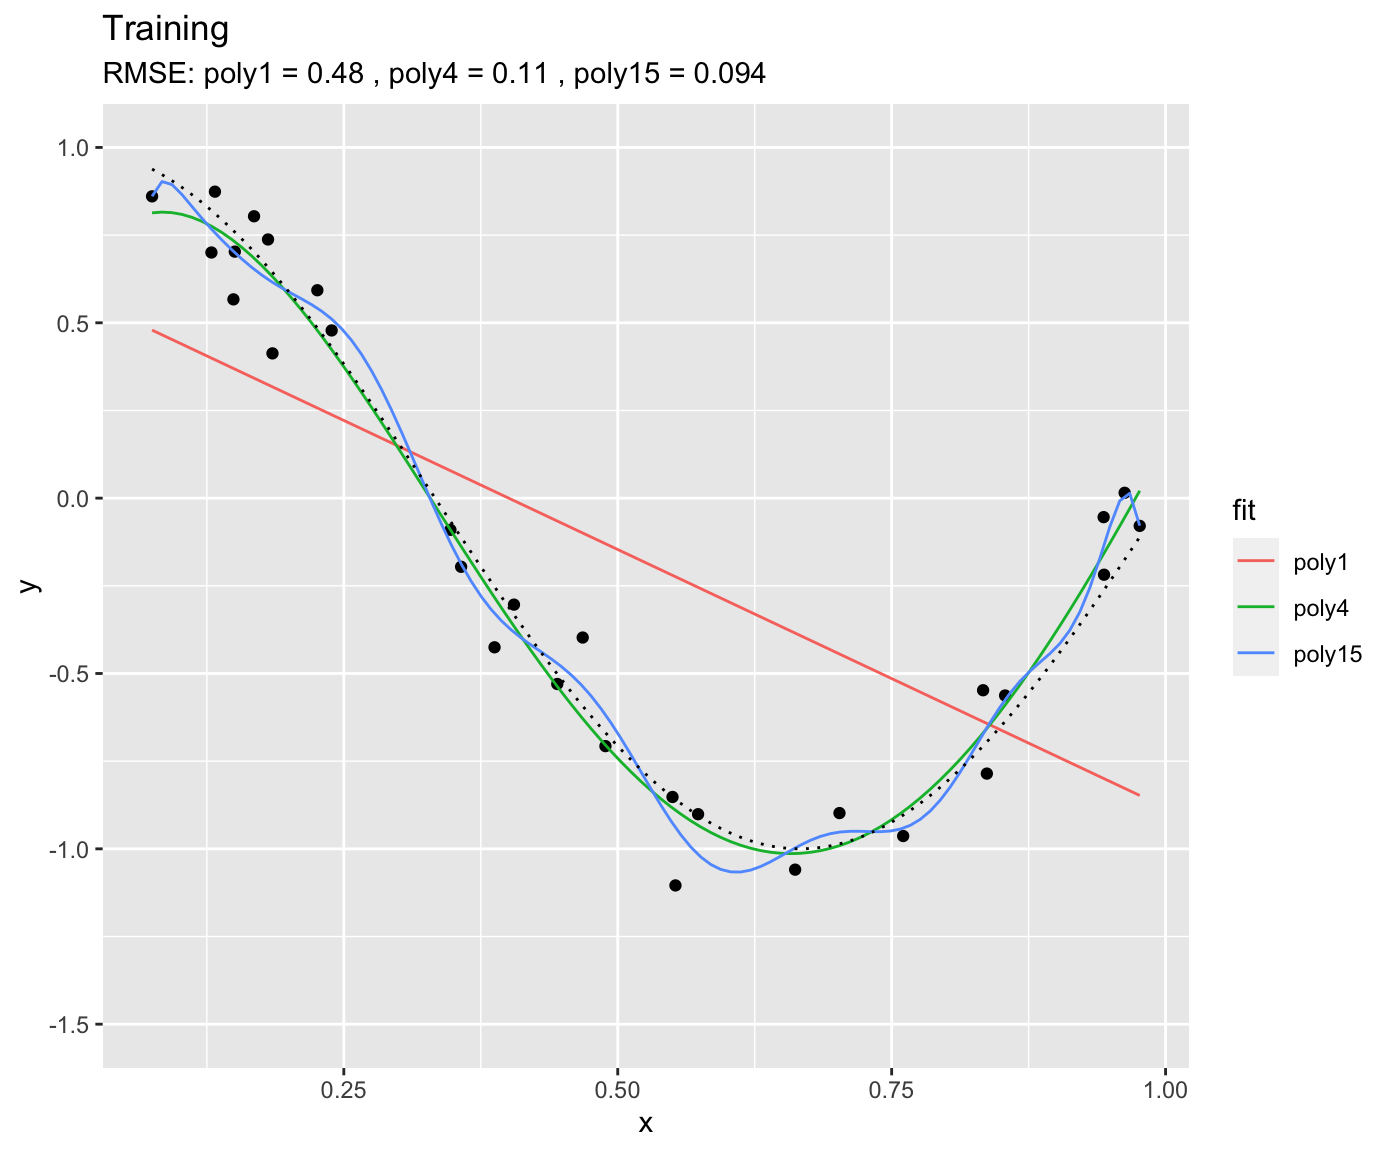
\includegraphics{ml4ec_workshop_files/figure-latex/unnamed-chunk-3-1} \end{center}

We can use the same fitted models on unseen data - the \emph{validation data}. This is what's done below. Again, the same true underlying relationship is used, but we sample a new set of data points in x and add a new sample of errors on top of the true relationship.

\begin{center}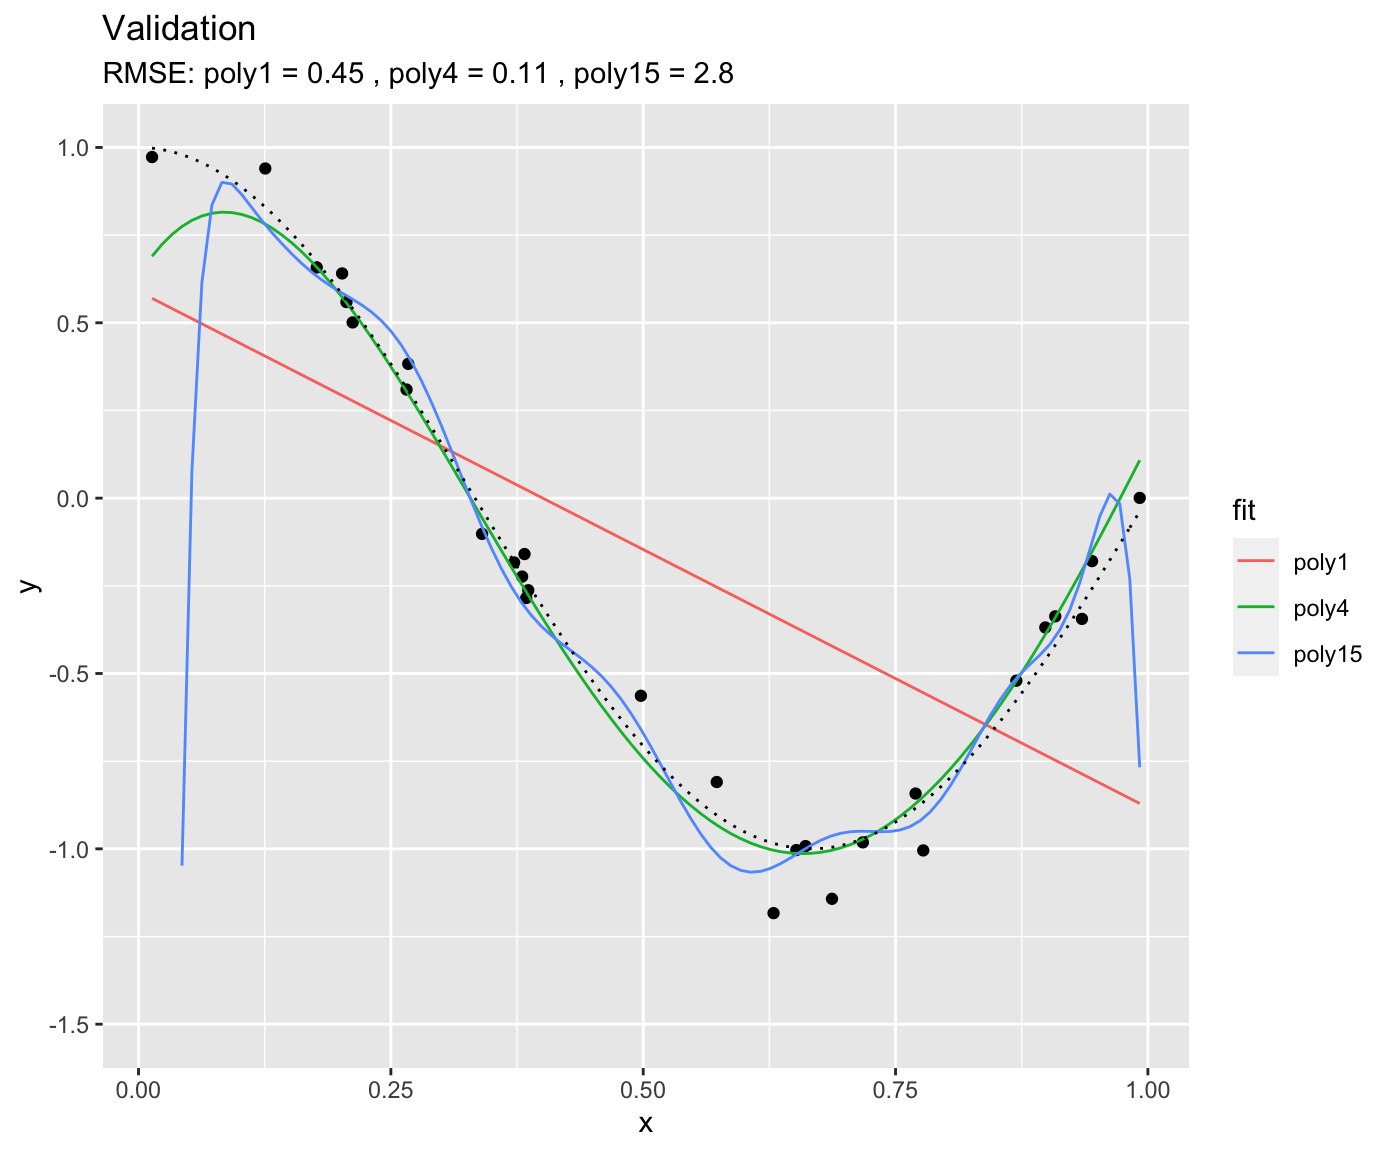
\includegraphics{ml4ec_workshop_files/figure-latex/unnamed-chunk-4-1} \end{center}

You see that, using the validation set, we find that ``poly4'' actually performs the best - it has a much lower RMSE that ``poly15''. Apparently, ``poly15'' was overfitted. Apparently, it indeed used its flexibility to fit not only the shape of the true underlying relationship, but also the observation errors on top of it. This has obviously the implication that, when this model is used to make predictions for data that was not used for training (calibration), it will yield misguided predictions that are affected by the errors in the training set. In the above pictures we can also conclude that ``poly1'' was underfitted.

It gets even worse when applying the fitted polynomial models to data that extends beyond the range in \(x\) that was used for model training. Here, we're extending just 20\% to the right.

\begin{center}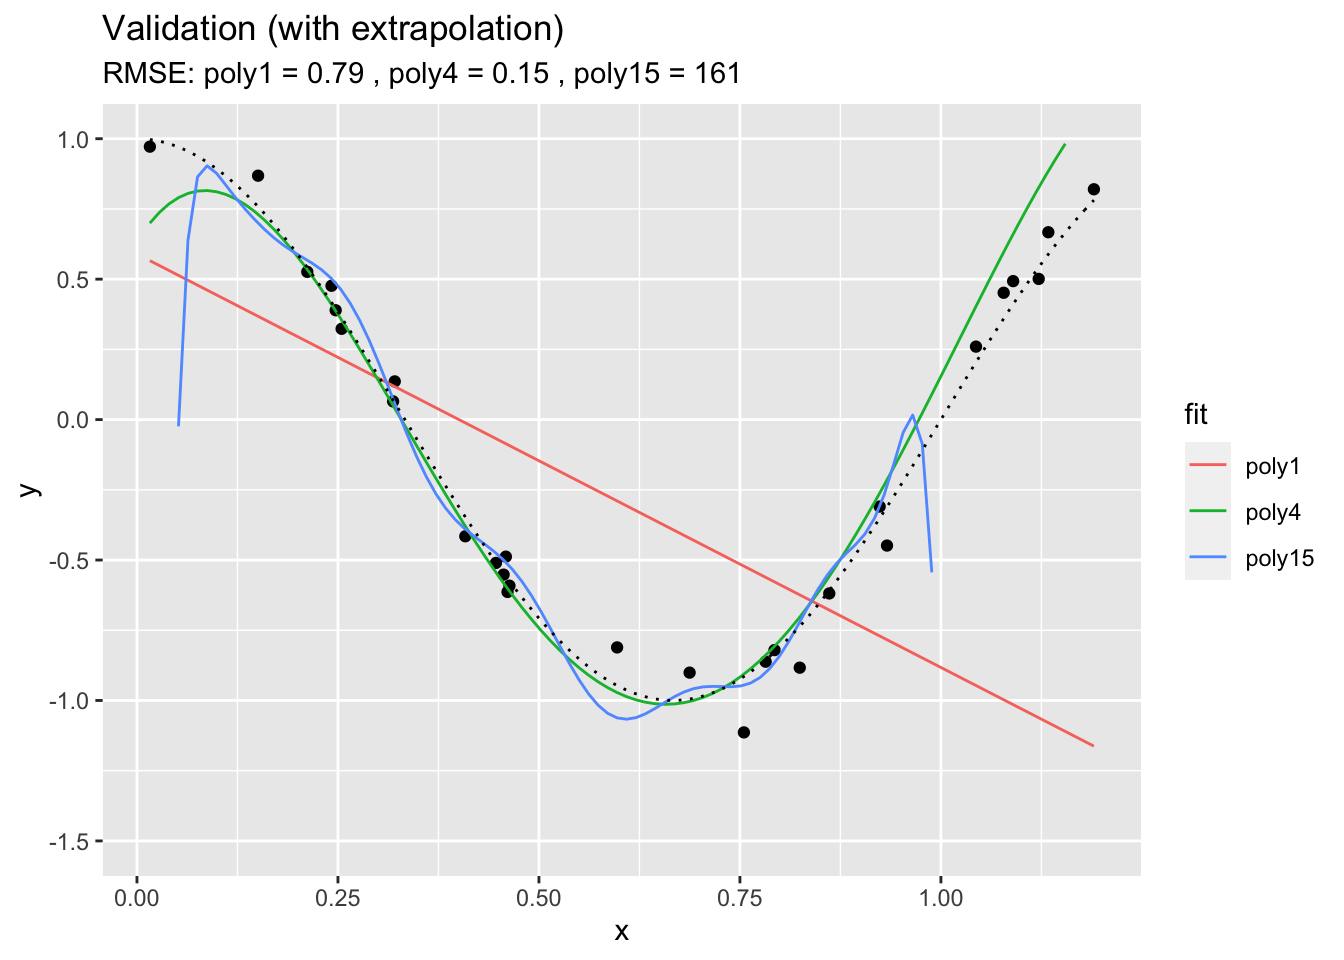
\includegraphics{ml4ec_workshop_files/figure-latex/unnamed-chunk-5-1} \end{center}

You see that the RMSE for ``poly15'' literally explodes. The model is hopelessly overfitted and completely useless for prediction, although it looked like it fit the data best when we considered at the training results. This is a fundamental challenge in ML - finding the model with the best \emph{generalisability}. That is, a model that not only fits the training data well, but also performs well on unseen data.

The phenomenon of fitting/overfitting as a function of the model ``flexibility'' is also referred to as \emph{bias vs.~variance trade-off}. The bias describes how well a model matches the training set (average error). A model with low bias will match the data set closely and vice versa. The variance describes how much a model changes when you train it using different portions of your data set. ``poly15'' has a high variance, but much of its variance is the result of misled training on observation errors. On the other extreme, ``poly1'' has a high bias. It's not affected by the noise in observations, but its predictions are also far off the observations. In ML, we are challenged to balance this trade-off. In Figure \ref{fig:tradeoff} you can see a schematic illustration of the bias--variance trade-off.

This chapter introduces the methods to achieve the best model generalisability and find the sweet spot between high bias and high variance. The steps to get there include the preprocessing of data, splitting the data into training and testing sets, and model training that ``steers'' the model towards what is considered a good model fit in terms of its generalisation power.

You have learned in video 6a about the basic setup of supervised ML, with input data containing the features (or predictors) \(X\), predicted (\(\hat{Y}\)) and observed target values (\(Y\), also known as \emph{labels}). In video 6b (title 6c: loss and it's minimization), you learned about the loss function which quantifies the agreement between \(Y\) and \(\hat{Y}\) and defines the objective of the model training. Here, you'll learn how all of this can be implemented in R. Depending on your application or research question, it may also be of interest to evaluate the relationships embodied in \(f(X)\) or to quantify the importance of different predictors in our model. This is referred to as \emph{model interpretation} and is introduced in the respectively named subsection. Finally, we'll get into \emph{feature selection} in the next Application session.

The topic of supervised machine learning methods covers enough material to fill two sessions. Therefore, we split this part in two. Model training, implementing the an entire modelling workflow, model evaluation and interpretation will be covered in the next session's tutorial (Supervised Machine Learning Methods II).

Of course, a plethora of algorithms exist that do the job of \(Y = f(X)\). Each of them has its own strengths and limitations. It is beyond the scope of this course to introduce a larger number of ML algorithms. Subsequent sessions will focus primarily on Artificial Neural Networks (ANN) - a type of ML algorithm that has gained popularity for its capacity to efficiently learn patterns in large data sets. For illustration purposes in this and the next chapter, we will briefly introduce two simple alternative ``ML'' methods, linear regression and K-nearest-neighbors. They have quite different characteristics and are therefore great for illustration purposes in this chapter.

\hypertarget{our-modelling-challenge}{%
\section{Our modelling challenge}\label{our-modelling-challenge}}

The environment determines ecosystem-atmosphere exchange fluxes of water vapour and CO2. Temporally changing mass exchange fluxes can be continuously measured with the eddy covariance technique, while abiotic variables (meteorological variables, soil moisture) can be measured in parallel. This offers an opportunity for building models that predict mass exchange fluxes from the environment.

In this workshop, we formulate a model for predicting ecosystem gross primary production (photosynthesis) from environmental covariates.

This is to say that \texttt{GPP\_NT\_VUT\_REF} is the target variable, and other available variables available in the dataset can be used as predictors.

\hypertarget{data}{%
\section{Data}\label{data}}

Data is provided here at daily resolution for a site (`CH-Dav') located in the Swiss alps (Davos). This is one of the longest-running eddy covariance sites globally and measures fluxes in a evergreen coniferous forest with cold winters and temperate and relatively moist summers.

For more information of the variables in the dataset, see \href{http://fluxnet.fluxdata.org/data/fluxnet2015-dataset/}{FLUXNET 2015 website}, and \href{https://www.nature.com/articles/s41597-020-0534-3}{Pastorello et al., 2020} for a comprehensive documentation of variable definitions and methods.

\hypertarget{available-variables}{%
\subsection{Available variables}\label{available-variables}}

\begin{itemize}
\tightlist
\item
  \texttt{TIMESTAMP}: Day of measurement.
\item
  \texttt{TA\_F}: Air temperature. The meaning of suffix \texttt{\_F} is described in \href{https://www.nature.com/articles/s41597-020-0534-3}{Pastorello et al., 2020}.
\item
  \texttt{SW\_IN\_F}: Shortwave incoming radiation
\item
  \texttt{LW\_IN\_F}: Longwave incoming radiation
\item
  \texttt{VPD\_F}: Vapour pressure deficit (relates to the humidity of the air)
\item
  \texttt{PA\_F}: Atmospheric pressure
\item
  \texttt{P\_F}: Precipitation
\item
  \texttt{WS\_F}: Wind speed
\item
  \texttt{GPP\_NT\_VUT\_REF}: Gross primary production - \textbf{the target variable}
\item
  \texttt{NEE\_VUT\_REF\_QC}: Quality control information for \texttt{GPP\_NT\_VUT\_REF}. Specifies the fraction of high-quality underlying high-frequency data from which the daily data is derived. 0.8 = 80\% underlying high-quality data, remaining 20\% of the high-frequency data is gap-filled.
\end{itemize}

\hypertarget{more-primers}{%
\section{More primers}\label{more-primers}}

\hypertarget{k-nearest-neighbours}{%
\subsection{K-nearest neighbours}\label{k-nearest-neighbours}}

As the name suggests, the K-nearest neighbour (KNN) uses the \(k\) observations that are ``nearest'' to the new record for which we want to make a prediction. It then calculates their average (in regression) or most frequent value (in classification) as the prediction. ``Nearest'' is determined by some distance metric evaluated based on the values of the predictors. In our example (\texttt{GPP\_NT\_VUT\_REF\ \textasciitilde{}\ .}), KNN would determine the \(k\) days where conditions, given by our set of predictors, were most similar (nearest) to the day for which we seek a prediction. Then, it calculates the prediction as the average (mean) GPP value of these days. Determining ``nearest'' neighbors is commonly based on either the Euclidean or Manhattan distances between two data points \(x_a\) and \(x_b\), considering all \(p\) predictors \(j\).

Euclidean distance:
\[
\sqrt{ \sum_{j=1}^p (x_{a,j} - x_{b,j})^2  } \\
\]
Manhattan distance:
\[
\sum_{j=1}^p | x_{a,j} - x_{b,j} |
\]

In two-dimensional space, the Euclidean distance measures the length of a straight line between two points (remember Pythagoras!). The Manhattan distance is called this way because it measures the distance you would have to walk to get from point \(a\) to point \(b\) in Manhattan, New York, where you cannot cut corners but have to follow a rectangular grid of streets. \(|x|\) is the positive value of \(x\) ( \(|-x| = x\)).

KNN is a simple algorithm that uses knowledge of the ``local'' data structure for prediction. A drawback is that the model training has to be done for each prediction step and the computation time of the training increases with \(x \times p\). KNNs are used, for example, to impute values (fill missing values) and have the advantage that predicted values are always within the range of observed values of the target variable.

\hypertarget{random-forest}{%
\subsection{Random Forest}\label{random-forest}}

Random forest models are based on \emph{decision trees}, where binary decisions for predicting the target's values are based on thresholds of the predictors' values. The \emph{depth} of a decision tree refers to the number of such decisions. The deeper a tree, the more likely the model will overfit. Here are some links for more information on decision trees:

\begin{itemize}
\tightlist
\item
  \href{https://bradleyboehmke.github.io/HOML/DT.html}{Hands On Machine-Learning in R}
\end{itemize}

Just as forests are made up by trees, \emph{random Forest} models make use of random subsets of the original data and of available predictions and respective decision trees. Predictions are then made by averaging predictions of individual \emph{base learners} (the decision trees). The number of predictors considered at each decision step is a tunable parameter (a \emph{hyperparameter}, typically called \(m_{try}\)). Introducing this randomness is effective because decision trees tend to overfit and because of the \emph{wisdom of the crowd} - i.e., the power of aggregating individual predictions with their random error (and without systematic bias) for generating accurate and relatively precise predictions.

Random forest models have gained particular popularity and are widely applied in environmental sciences not only for their power, but also for their ease of use. No preprocessing (centering, scaling) is necessary, they can deal with skewed data, and can effectively learn interactions between predictors.

Here are some links for more information on random forest:

\begin{itemize}
\tightlist
\item
  \href{https://bradleyboehmke.github.io/HOML/random-forest.html}{Hands On Machine-Learning in R}
\end{itemize}

\hypertarget{data-splitting}{%
\chapter{Data splitting}\label{data-splitting}}

\hypertarget{reading-and-wrangling-data}{%
\section{Reading and wrangling data}\label{reading-and-wrangling-data}}

Let's start by reading our data and apply few processing steps (\emph{wrangling}).

There is a difference between data wrangling and pre-processing as part of the modelling workflow, which we will learn about in Chapter \ref{preprocessing}. Data wrangling can be considered to encompass the steps to prepare the data set prior to modelling, including, combining variables from different sources, removal of bad or missing data, and aggregating to the desired resolution or granularity (e.g., averaging over all time steps in a day, or over all replicates in a sample). See the \href{https://github.com/Quartz/bad-data-guide}{Quartz Guide to Bad Data} for an overview of how to deal with different types of bad data.

In contrast, \emph{pre-processing} refers to the additional steps that are either required by the ML algorithm (e.g.~centering and scaling for KNN or neural networks) or the transformation of variables guided by the resulting improvement of the predictive power of the ML model. In other words, pre-processing is part of the modelling workflow and includes all steps that apply transformations that use parameters derived from the data.

We are provided with a data file in the format of comma-separated-values (CSV), obtained through \href{https://fluxnet.org/data/fluxnet2015-dataset/}{FLUXNET2015}. It contains data from one site (\href{https://gl.ethz.ch/infrastructure/sites/davos.html}{CH-Dav}) at a daily time step, and includes quality control information for each variable.

Let's read the data, select relevant variables, convert the time stamp column to a time object and interpret missing values (encoded \texttt{-9999} in the file).

\begin{Shaded}
\begin{Highlighting}[]
\FunctionTok{library}\NormalTok{(tidyverse)}

\NormalTok{ddf }\OtherTok{\textless{}{-}} \FunctionTok{read\_csv}\NormalTok{(}\StringTok{"./data/FLX\_CH{-}Dav\_FLUXNET2015\_FULLSET\_DD\_1997{-}2014\_1{-}3.csv"}\NormalTok{) }\SpecialCharTok{\%\textgreater{}\%} 
  
  \DocumentationTok{\#\# select only the variables we are interested in}
  \FunctionTok{select}\NormalTok{(TIMESTAMP,}
\NormalTok{         GPP\_NT\_VUT\_REF,    }\CommentTok{\# the target}
\NormalTok{         NEE\_VUT\_REF\_QC,    }\CommentTok{\# quality control info}
         \FunctionTok{ends\_with}\NormalTok{(}\StringTok{"\_F"}\NormalTok{),   }\CommentTok{\# includes all all meteorological variables}
         \SpecialCharTok{{-}}\FunctionTok{contains}\NormalTok{(}\StringTok{"JSB"}\NormalTok{)   }\CommentTok{\# weird useless variable}
\NormalTok{         ) }\SpecialCharTok{\%\textgreater{}\%}

  \DocumentationTok{\#\# convert to a nice date object}
  \FunctionTok{mutate}\NormalTok{(}\AttributeTok{TIMESTAMP =}\NormalTok{ lubridate}\SpecialCharTok{::}\FunctionTok{ymd}\NormalTok{(TIMESTAMP)) }\SpecialCharTok{\%\textgreater{}\%}

  \DocumentationTok{\#\# set all {-}9999 to NA}
  \FunctionTok{na\_if}\NormalTok{(}\SpecialCharTok{{-}}\DecValTok{9999}\NormalTok{) }\SpecialCharTok{\%\textgreater{}\%}

  \DocumentationTok{\#\# drop QC variables (no longer needed), except NEE\_VUT\_REF\_QC}
  \FunctionTok{select}\NormalTok{(}\SpecialCharTok{{-}}\FunctionTok{ends\_with}\NormalTok{(}\StringTok{"\_QC"}\NormalTok{), NEE\_VUT\_REF\_QC)}
\end{Highlighting}
\end{Shaded}

If the style of the code above looks unfamiliar - this is the \textbf{\href{https://www.tidyverse.org/}{tidyverse}}. The tidyverse is a R syntax ``dialect'' and a collection of R functions and packages. They share the structure of arguments and function return values than can be combined to a chain by the \texttt{\%\textgreater{}\%} (``pipe'') operator. For this, the output of each function is a data frame which is ``piped'' to the next function, and each function takes a data frame as input. What is piped into a function takes the place of the first argument, normally provided in brackets. This enables ease with typical data wrangling and visualization tasks (\textbf{\href{https://ggplot2.tidyverse.org/}{ggplot2}} is part of it). This tutorial is generally written using tidyverse packages and code syntax.

The column \texttt{NEE\_VUT\_REF\_QC} provides information about the fraction of gap-filled half-hourly data used to calculate daily aggregates. Let's remove \texttt{GPP\_NT\_VUT\_REF} data, where more than 80\% of the half-hourly data was gap-filled. Make sure to not actually remove the respective rows, but rather replace values with NA.

\begin{Shaded}
\begin{Highlighting}[]
\NormalTok{ddf }\OtherTok{\textless{}{-}}\NormalTok{ ddf }\SpecialCharTok{\%\textgreater{}\%} 
  \FunctionTok{mutate}\NormalTok{(}\AttributeTok{GPP\_NT\_VUT\_REF =} \FunctionTok{ifelse}\NormalTok{(NEE\_VUT\_REF\_QC }\SpecialCharTok{\textless{}} \FloatTok{0.8}\NormalTok{, }\ConstantTok{NA}\NormalTok{, GPP\_NT\_VUT\_REF))}
\end{Highlighting}
\end{Shaded}

At this stage, we won't use \texttt{NEE\_VUT\_REF\_QC} any longer. So we can drop it.

\begin{Shaded}
\begin{Highlighting}[]
\NormalTok{ddf }\OtherTok{\textless{}{-}}\NormalTok{ ddf }\SpecialCharTok{\%\textgreater{}\%} 
  \FunctionTok{select}\NormalTok{(}\SpecialCharTok{{-}}\NormalTok{NEE\_VUT\_REF\_QC)}
\end{Highlighting}
\end{Shaded}

\hypertarget{splitting-into-testing-and-training-sets}{%
\section{Splitting into testing and training sets}\label{splitting-into-testing-and-training-sets}}

The introductory example impressively demonstrated the importance of validating the fitted model with data that was \emph{not} used for training. Thus, we can test the model's \emph{generalisability.} The essential step that enables us to assess the model's \emph{generalization error} is to hold out part of the data from training, and set it aside (leaving it absolutely untouched) for \emph{testing}.

There is no fixed rule for how much data are to be used for training and testing, respectively. We have to balance the trade-off between:

\begin{itemize}
\tightlist
\item
  Spending too much data for training will leave us with too little data for testing and the test results may not be robust. In this case, the sample size for getting robust validation statistics is not sufficiently large and we don't know for sure whether we are safe from an over-fit model.
\item
  Spending too much data for validation will leave us with too little data for training. In this case, the ML algorithm may not be successful at finding real relationships due to insufficient amounts of training data.
\end{itemize}

Typical splits are between 60-80\% for training. However, in cases where the number of data points is very large, the gains from having more training data are marginal, but come at the cost of adding to the already high computational burden of model training.

In environmental sciences, the number of predictors is often smaller than the sample size (\(p < n\)), because its typically easier to collect repeated observations of a particular variable than to expand the set of variables being observed. Nevertheless, in cases where the number \(p\) gets large, it is important, and for some algorithms mandatory, to maintain \(p < n\) for model training.

An important aspect to consider when splitting the data is to make sure that all ``states'' of the system for which we have data are approximately equally represented in training and testing sets. This is to make sure that the algorithm learns relationships \(f(X)\) also under rare conditions \(X\), for example meteorological extreme events.

Several alternative functions for the data splitting step are available from different packages in R. We will use the the \textbf{rsample} package as it allows to additionally make sure that data from the full range of a given variable's values (\texttt{VPD\_F} in the example below) are well covered in both training and testing sets.

\begin{Shaded}
\begin{Highlighting}[]
\FunctionTok{library}\NormalTok{(rsample)}
\FunctionTok{set.seed}\NormalTok{(}\DecValTok{123}\NormalTok{)  }\CommentTok{\# for reproducibility}
\NormalTok{split }\OtherTok{\textless{}{-}} \FunctionTok{initial\_split}\NormalTok{(ddf, }\AttributeTok{prop =} \FloatTok{0.7}\NormalTok{, }\AttributeTok{strata =} \StringTok{"VPD\_F"}\NormalTok{)}
\NormalTok{ddf\_train }\OtherTok{\textless{}{-}} \FunctionTok{training}\NormalTok{(split)}
\NormalTok{ddf\_test }\OtherTok{\textless{}{-}} \FunctionTok{testing}\NormalTok{(split)}
\end{Highlighting}
\end{Shaded}

Plot the distribution of values in the training and testing sets.

\begin{Shaded}
\begin{Highlighting}[]
\NormalTok{ddf\_train }\SpecialCharTok{\%\textgreater{}\%} 
  \FunctionTok{mutate}\NormalTok{(}\AttributeTok{split =} \StringTok{"train"}\NormalTok{) }\SpecialCharTok{\%\textgreater{}\%} 
  \FunctionTok{bind\_rows}\NormalTok{(ddf\_test }\SpecialCharTok{\%\textgreater{}\%} 
    \FunctionTok{mutate}\NormalTok{(}\AttributeTok{split =} \StringTok{"test"}\NormalTok{)) }\SpecialCharTok{\%\textgreater{}\%} 
  \FunctionTok{pivot\_longer}\NormalTok{(}\AttributeTok{cols =} \DecValTok{2}\SpecialCharTok{:}\DecValTok{9}\NormalTok{, }\AttributeTok{names\_to =} \StringTok{"variable"}\NormalTok{, }\AttributeTok{values\_to =} \StringTok{"value"}\NormalTok{) }\SpecialCharTok{\%\textgreater{}\%} 
  \FunctionTok{ggplot}\NormalTok{(}\FunctionTok{aes}\NormalTok{(}\AttributeTok{x =}\NormalTok{ value, }\AttributeTok{y =}\NormalTok{ ..density.., }\AttributeTok{color =}\NormalTok{ split)) }\SpecialCharTok{+}
  \FunctionTok{geom\_density}\NormalTok{() }\SpecialCharTok{+}
  \FunctionTok{facet\_wrap}\NormalTok{(}\SpecialCharTok{\textasciitilde{}}\NormalTok{variable, }\AttributeTok{scales =} \StringTok{"free"}\NormalTok{)}
\end{Highlighting}
\end{Shaded}

\begin{center}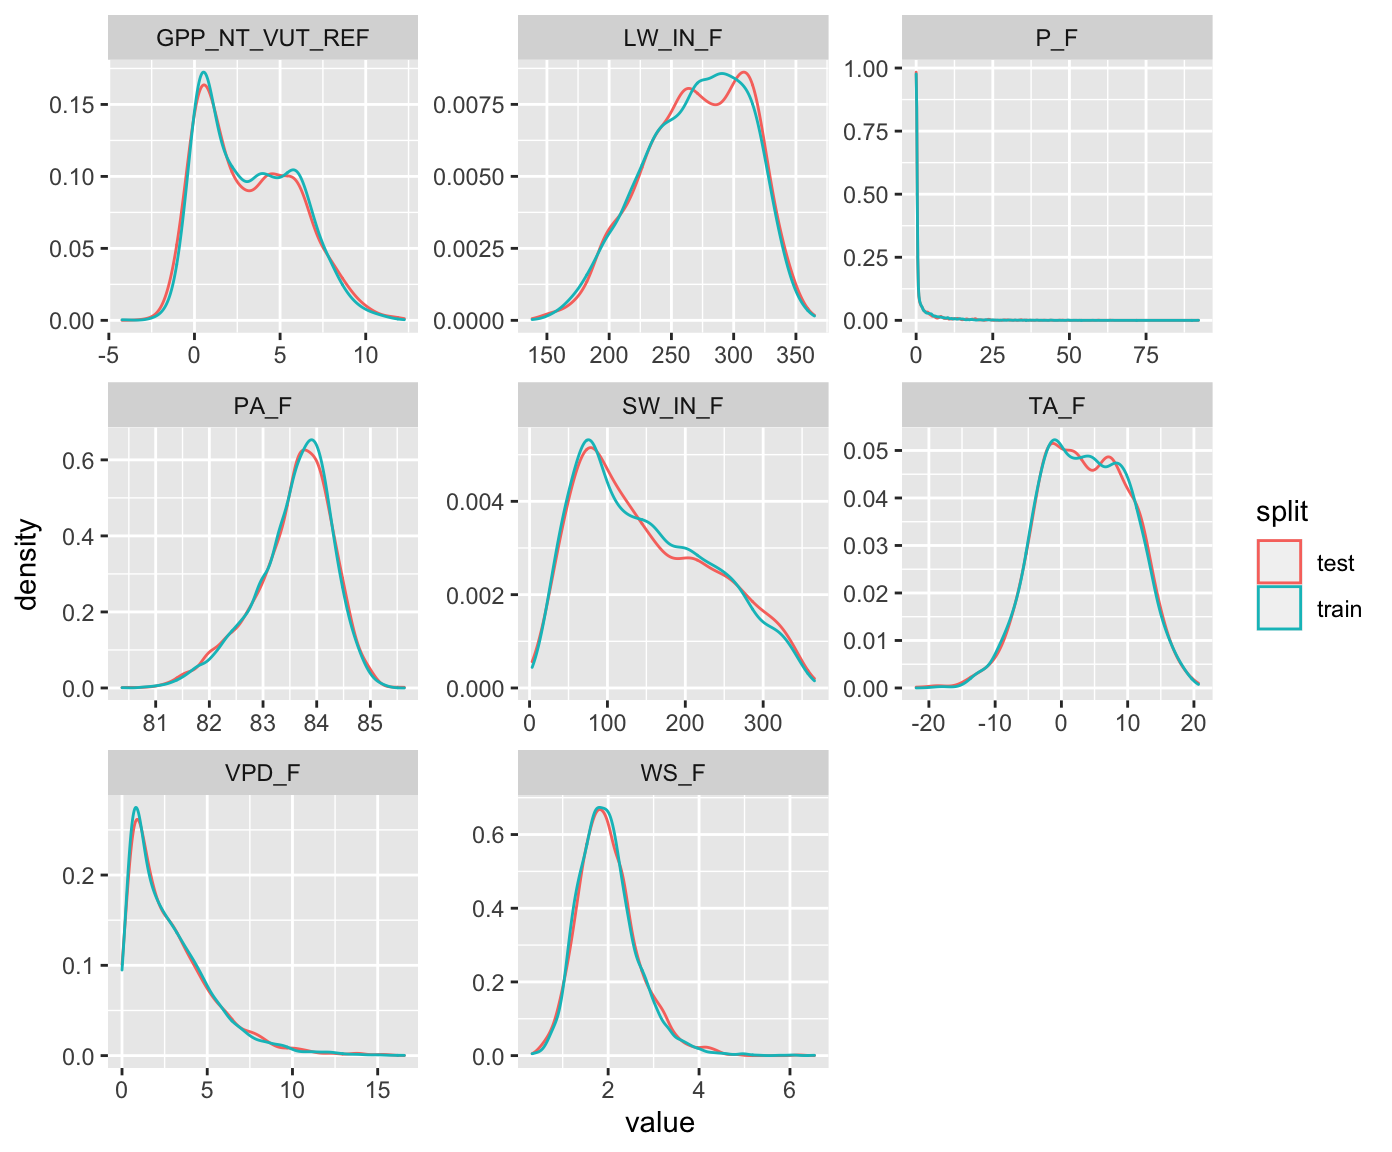
\includegraphics{ml4ec_workshop_files/figure-latex/unnamed-chunk-12-1} \end{center}

\hypertarget{preprocessing}{%
\chapter{Pre-processing}\label{preprocessing}}

Skewed data, outliers, and values covering multiple orders of magnitude can create difficulties for certain ML algorithms, e.g., or K-nearest neighbours, or neural networks. Other algorithms, like tree-based methods (e.g., Random Forest), are more robust against such issues.

\hypertarget{dealing-with-missingness-and-bad-data}{%
\section{Dealing with missingness and bad data}\label{dealing-with-missingness-and-bad-data}}

Several ML algorithms require missing values to be removed. That is, if any of the cells in one row has a missing value, the entire cell gets removed. Data may be missing for several reasons. Some yield random patterns of missing data, others not. In the latter case, we can speak of \emph{informative missingness} (Kuhn \& Johnson, 2003) and its information can be used for predictions. For categorical data, we may replace such data with \texttt{"none"} (instead of \texttt{NA}), while randomly missing data may be dropped altogether. Some ML algorithms (mainly tree-based methods, e.g., random forest) can handle missing values. However, when comparing the performance of alternative ML algorithms, they should be tested with the same data and removing missing data should be done beforehand.

Visualising missing data is essential for making decisions about dropping rows with missing data versus removing predictors from the model (which would imply too much data removal). The cells with missing data in a data frame can be eaily visualised e.g.~with \texttt{vis\_miss()} from the \emph{visdat} package.

\begin{Shaded}
\begin{Highlighting}[]
\FunctionTok{library}\NormalTok{(visdat)}
\FunctionTok{vis\_miss}\NormalTok{(}
\NormalTok{  ddf,}
  \AttributeTok{cluster =} \ConstantTok{FALSE}\NormalTok{, }
  \AttributeTok{warn\_large\_data =} \ConstantTok{FALSE}
\NormalTok{  )}
\end{Highlighting}
\end{Shaded}

\begin{center}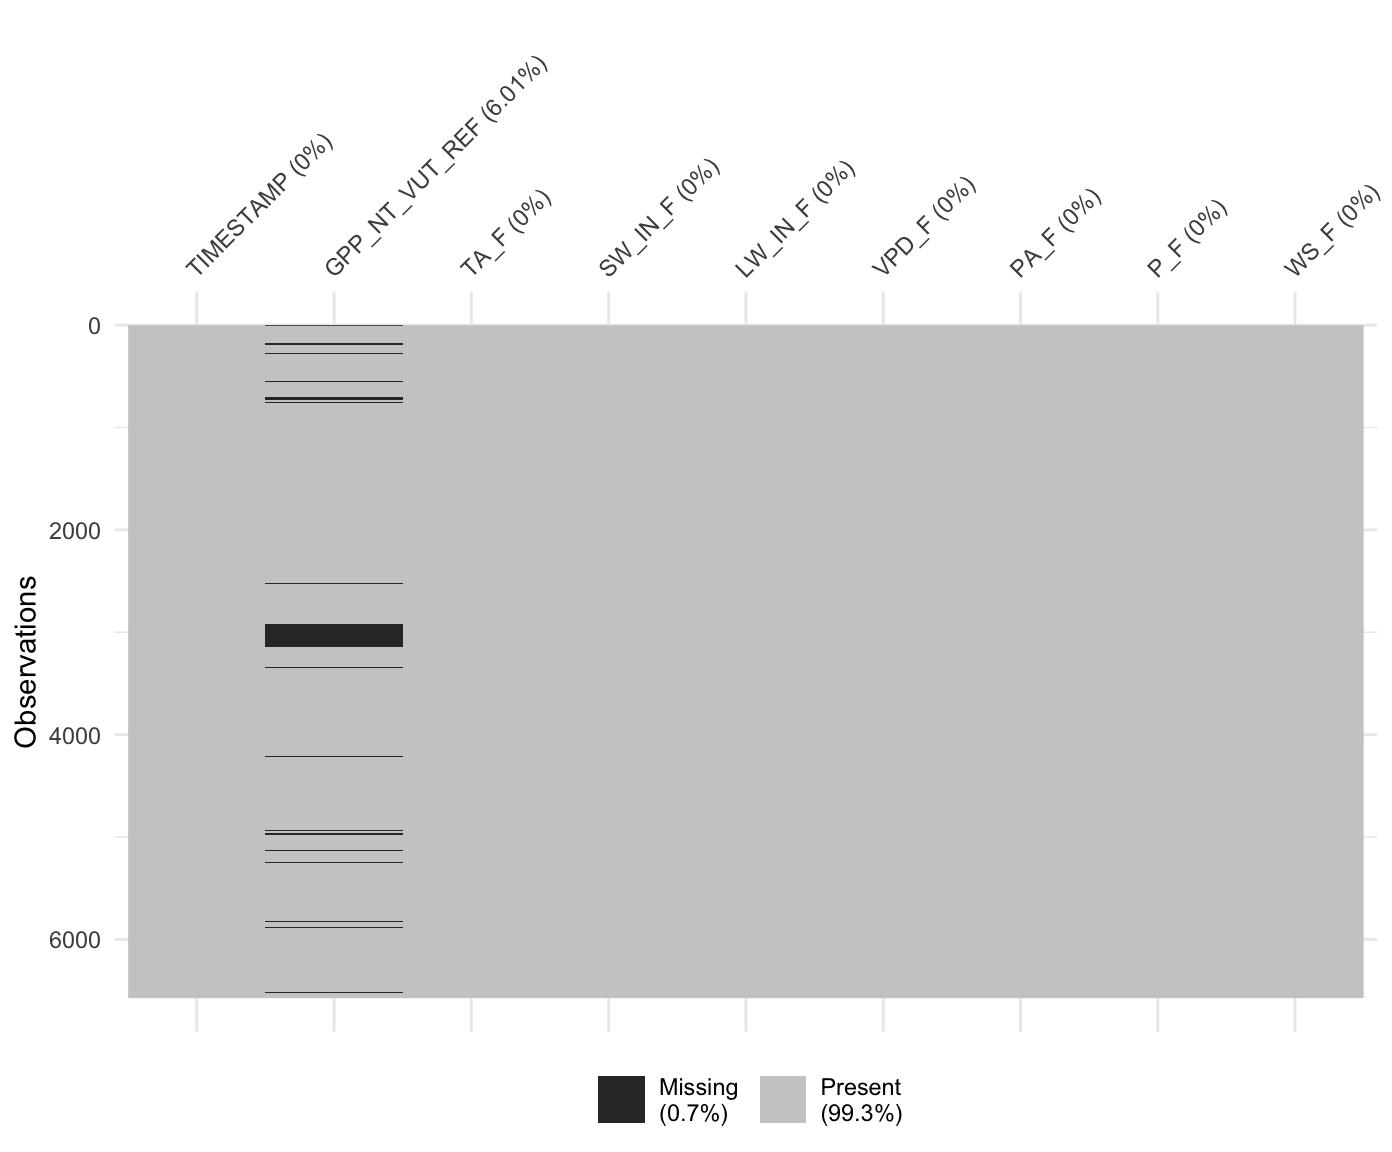
\includegraphics{ml4ec_workshop_files/figure-latex/unnamed-chunk-14-1} \end{center}

The question about what is ``bad data'' and whether or when it should be removed is often critical. Such decisions are important to keep track of and should be reported as transparently as possible in publications. In reality, where the data generation process may start in the field with actual human beings writing notes in a lab book, and where the human collecting the data is often not the same as the human writing the paper, it's often more difficult to keep track of such decisions. As a general principle, it is advisable to design data records such that decisions made during its process remain transparent throughout all stages of the workflow and that sufficient information be collected to enable later revisions of particularly critical decisions.

\hypertarget{standardization}{%
\section{Standardization}\label{standardization}}

Several algorithms explicitly require data to be standardized. That is, values of all predictors vary within a comparable range. The necessity of this step becomes obvious when considering neural networks, the activation functions of each node have to deal with standardized inputs. In other words, inputs have to vary over the same range, expecting a mean of zero and standard deviation of one.)

To get a quick overview of the distribution of all variables (columns) in our data frame, we can use the \emph{skimr} package.

\begin{Shaded}
\begin{Highlighting}[]
\FunctionTok{library}\NormalTok{(skimr)}
\NormalTok{knitr}\SpecialCharTok{::}\FunctionTok{kable}\NormalTok{(}\FunctionTok{skim}\NormalTok{(ddf))}
\end{Highlighting}
\end{Shaded}

\begin{tabular}{l|l|r|r|l|l|l|r|r|r|r|r|r|r|r|l}
\hline
skim\_type & skim\_variable & n\_missing & complete\_rate & Date.min & Date.max & Date.median & Date.n\_unique & numeric.mean & numeric.sd & numeric.p0 & numeric.p25 & numeric.p50 & numeric.p75 & numeric.p100 & numeric.hist\\
\hline
Date & TIMESTAMP & 0 & 1.0000000 & 1997-01-01 & 2014-12-31 & 2005-12-31 & 6574 & NA & NA & NA & NA & NA & NA & NA & NA\\
\hline
numeric & GPP\_NT\_VUT\_REF & 395 & 0.9399148 & NA & NA & NA & NA & 3.218728 & 2.7569372 & -4.22996 & 0.7730585 & 2.87334 & 5.44718 & 12.2567 & ▁▇▆▃▁\\
\hline
numeric & TA\_F & 0 & 1.0000000 & NA & NA & NA & NA & 3.517397 & 6.6562542 & -21.92400 & -1.5565000 & 3.44450 & 8.72200 & 20.6870 & ▁▂▇▇▂\\
\hline
numeric & SW\_IN\_F & 0 & 1.0000000 & NA & NA & NA & NA & 150.785747 & 85.0156424 & 3.30300 & 78.2630000 & 136.67700 & 215.54125 & 365.8880 & ▆▇▆▅▂\\
\hline
numeric & LW\_IN\_F & 0 & 1.0000000 & NA & NA & NA & NA & 269.771156 & 41.9073945 & 138.12500 & 239.3937500 & 272.62150 & 303.36150 & 364.9070 & ▁▃▇▇▂\\
\hline
numeric & VPD\_F & 0 & 1.0000000 & NA & NA & NA & NA & 2.865737 & 2.3936778 & 0.00100 & 0.9950000 & 2.23900 & 4.05775 & 16.5650 & ▇▃▁▁▁\\
\hline
numeric & PA\_F & 0 & 1.0000000 & NA & NA & NA & NA & 83.564688 & 0.7261651 & 80.37300 & 83.1600000 & 83.68300 & 84.07200 & 85.6330 & ▁▁▅▇▁\\
\hline
numeric & P\_F & 0 & 1.0000000 & NA & NA & NA & NA & 2.304499 & 5.7860345 & 0.00000 & 0.0000000 & 0.00000 & 1.60000 & 92.1000 & ▇▁▁▁▁\\
\hline
numeric & WS\_F & 0 & 1.0000000 & NA & NA & NA & NA & 1.991029 & 0.6604529 & 0.32800 & 1.5410000 & 1.92200 & 2.33900 & 6.5390 & ▃▇▁▁▁\\
\hline
\end{tabular}

We see for example, that typical values of \texttt{LW\_IN\_F} are by a factor 100 larger than values of \texttt{VPD\_F}. KNN uses the distance from neighbouring points for predictions. Obviously, in this case here, any distance would be dominated by \texttt{LW\_IN\_F} and distances in the ``direction'' of \texttt{VPD\_F}, even when relatively large, would not be influential, neither for a Euclidean nor a Manhattan distance (see \ref{introduction}). In neural networks, activation functions take values in a given range (0-1). Thus, for both algorithms, data has to be standardized prior to model training.

Standardization is done, for example, by dividing each variable, that is all values in one column, by the standard deviation of that variable, and then subtracting its mean. This way, the resulting standardized values are centered around 0, and scaled such that a value of 1 means that the data point is one standard deviation above the mean of the respective variable (column). When applied to all predictors individually, the absolute values of their variations can be directly compared and only then it can be meaningfully used for determining the distance.

Standardization can be done not only by centering and scaling (as described above), but also by \emph{scaling to within range}, where values are scaled such that the minimum value within each variable (column) is 0 and the maximum is 1.

In order to avoid \emph{data leakage}, centering and scaling has to be done separately for each split into training and validation data (more on that later). In other words, don't center and scale the entire data frame with the mean and standard deviation derived from the entire data frame, but instead center and scale with mean and standard deviation derived from the training portion of the data, and apply that also to the validation portion, when evaluating.

The \emph{caret} package takes care of this. The R package \href{https://topepo.github.io/caret/}{\textbf{caret}} provides a unified interface for using different ML algorithms implemented in separate packages. The preprocessing steps applied with each resampling fold can be specified using the function \texttt{preProcess()}. More on resampling in Chapter \ref{training}.

\begin{Shaded}
\begin{Highlighting}[]
\FunctionTok{library}\NormalTok{(caret)}
\NormalTok{pp }\OtherTok{\textless{}{-}} \FunctionTok{preProcess}\NormalTok{(ddf\_train, }\AttributeTok{method =} \FunctionTok{c}\NormalTok{(}\StringTok{"center"}\NormalTok{, }\StringTok{"scale"}\NormalTok{))}
\end{Highlighting}
\end{Shaded}

As seen above for the feature engineering example, this does not return a standardized version of the data frame \texttt{ddf}. Rather, it returns the information that allows us to apply the same standardization also to other data sets. In other words, we use the distribution of values in the data set to which we applied the function to determine the centering and scaling (here: mean and standard deviation).

\hypertarget{more-pre-processing}{%
\section{More pre-processing}\label{more-pre-processing}}

Depending on the algorithm and the data, additional pre-processing steps may be required. You can find more information about this in the great and freely available online tutorial \href{https://bradleyboehmke.github.io/HOML/engineering.html\#target-engineering}{Hands-On Machine Learning in R}.

One such additional pre-processing step is \emph{imputation}, where missing values are imputed (gap-filled), for example by the mean of each variable respectively. Also imputation is prone to cause data leakage and must therefore be implemented as part of the resampling and training workflow. The \textbf{recipes} package offers a great way to deal with imputation (and also all other pre-processing steps). \href{https://bradleyboehmke.github.io/HOML/engineering.html\#impute}{Here} is a link to learn more about it.

\hypertarget{model-formulation}{%
\chapter{Model formulation}\label{model-formulation}}

The aim of supervised ML is to find a model \(\hat{Y} = f(X)\) so that \(\hat{Y}\) agrees well with observations \(Y\). We typically start with a research question where \(Y\) is given - naturally - by the problem we are addressing and we have a data set at hand where one or multiple predictors (or features) \(X\) are recorded along with \(Y\). From our data, we have information about how GPP (ecosystem-level photosynthesis) depends on set of abiotic factors, mostly meteorological measurements.

\hypertarget{formula-notation}{%
\section{Formula notation}\label{formula-notation}}

In R, it is common to use the \emph{formula} notation to specify the target and predictor variables. You have probably encountered formulas before, e.g., for a linear regression using the \texttt{lm()} function. To specify a linear regression model for \texttt{GPP\_NT\_VUT\_REF} with three predictors \texttt{SW\_F\_IN}, \texttt{VPD\_F}, and \texttt{TA\_F}, we write:

\begin{Shaded}
\begin{Highlighting}[]
\FunctionTok{lm}\NormalTok{(GPP\_NT\_VUT\_REF }\SpecialCharTok{\textasciitilde{}}\NormalTok{ SW\_F\_IN }\SpecialCharTok{+}\NormalTok{ VPD\_F }\SpecialCharTok{+}\NormalTok{ TA\_F, }\AttributeTok{data =}\NormalTok{ ddf)}
\end{Highlighting}
\end{Shaded}

\hypertarget{the-generic-train}{%
\section{\texorpdfstring{The generic \texttt{train()}}{The generic train()}}\label{the-generic-train}}

Actually, the way we formulate a model is independent of the algorithm, or \emph{engine} that takes care of fitting \(f(X)\). As mentioned in Chapter \ref{preprocessing} the R package \href{https://topepo.github.io/caret/}{\textbf{caret}} provides a unified interface for using different ML algorithms implemented in separate packages. In other words, it acts as a \emph{wrapper} for multiple different model fitting, or ML algorithms. This has the advantage that it unifies the interface (the way arguments are provided). caret also provides implementations for a set of commonly used tools for data processing, model training, and evaluation. We'll use caret for model training with the function \texttt{train()} (more on model training in Chapter \ref{training}). Note however, that using a specific algorithm, which is implemented in a specific package outside caret, also requires that the respective package be installed and loaded. Using caret for specifying the same linear regression model as above, the base-R \texttt{lm()} function, can be done with caret in a generalized form as:

\begin{Shaded}
\begin{Highlighting}[]
\FunctionTok{library}\NormalTok{(caret)}
\FunctionTok{train}\NormalTok{(}
  \AttributeTok{form =}\NormalTok{ GPP\_NT\_VUT\_REF }\SpecialCharTok{\textasciitilde{}}\NormalTok{ SW\_IN\_F }\SpecialCharTok{+}\NormalTok{ VPD\_F }\SpecialCharTok{+}\NormalTok{ TA\_F, }
  \AttributeTok{data =}\NormalTok{ ddf }\SpecialCharTok{\%\textgreater{}\%} \FunctionTok{drop\_na}\NormalTok{(), }
  \AttributeTok{method =} \StringTok{"lm"}
\NormalTok{)}
\end{Highlighting}
\end{Shaded}

\begin{verbatim}
## Linear Regression 
## 
## 6179 samples
##    3 predictor
## 
## No pre-processing
## Resampling: Bootstrapped (25 reps) 
## Summary of sample sizes: 6179, 6179, 6179, 6179, 6179, 6179, ... 
## Resampling results:
## 
##   RMSE      Rsquared   MAE     
##   1.599712  0.6646581  1.241035
## 
## Tuning parameter 'intercept' was held constant at a value of TRUE
\end{verbatim}

Of course, this is an overkill compared to just writing \texttt{lm(...)}. But the advantage of the unified interface is that we can simply replace the \texttt{method} argument to use a different ML algorithm. For example, to use a random forest model implemented by the \textbf{ranger} package, we can write:

\begin{Shaded}
\begin{Highlighting}[]
\DocumentationTok{\#\# do not run}
\FunctionTok{train}\NormalTok{(}
  \AttributeTok{form =}\NormalTok{ GPP\_NT\_VUT\_REF }\SpecialCharTok{\textasciitilde{}}\NormalTok{ SW\_F\_IN }\SpecialCharTok{+}\NormalTok{ VPD\_F }\SpecialCharTok{+}\NormalTok{ TA\_F, }
  \AttributeTok{data =}\NormalTok{ ddf, }
  \AttributeTok{method =} \StringTok{"ranger"}\NormalTok{,}
\NormalTok{  ...}
\NormalTok{)}
\end{Highlighting}
\end{Shaded}

The \texttt{...} hints at the fact that there are a few more arguments to be specified for training a random forest model with ranger. More on that in Chapter \ref{training}.

\hypertarget{recipes}{%
\section{Recipes}\label{recipes}}

The \href{https://recipes.tidymodels.org/}{\textbf{recipes}} package provides another way to specify the \emph{formula} and pre-processing steps in one go and is compatible with caret's \texttt{train()} function. For the same formula as above, and an example where the data \texttt{ddf\_train} is to be centered and scaled, we can specify the ``recipe'' using the \emph{tidyverse}-style pipe operator as:

\begin{Shaded}
\begin{Highlighting}[]
\FunctionTok{library}\NormalTok{(recipes)}
\NormalTok{pp }\OtherTok{\textless{}{-}} \FunctionTok{recipe}\NormalTok{(GPP\_NT\_VUT\_REF }\SpecialCharTok{\textasciitilde{}}\NormalTok{ SW\_IN\_F }\SpecialCharTok{+}\NormalTok{ VPD\_F }\SpecialCharTok{+}\NormalTok{ TA\_F, }\AttributeTok{data =}\NormalTok{ ddf\_train) }\SpecialCharTok{\%\textgreater{}\%} 
  \FunctionTok{step\_center}\NormalTok{(}\FunctionTok{all\_numeric}\NormalTok{(), }\SpecialCharTok{{-}}\FunctionTok{all\_outcomes}\NormalTok{()) }\SpecialCharTok{\%\textgreater{}\%}
  \FunctionTok{step\_scale}\NormalTok{(}\FunctionTok{all\_numeric}\NormalTok{(), }\SpecialCharTok{{-}}\FunctionTok{all\_outcomes}\NormalTok{())}
\end{Highlighting}
\end{Shaded}

The first line assigns \emph{roles} to the different variables. \texttt{GPP\_NT\_VUT\_REF} is an \emph{outcome} (in ``recipes speak''). Then, we used selectors to apply the recipe step to several variables at once. The first selector, \texttt{all\_numeric()}, selects all variables that are either integers or real values. The second selector, \texttt{-all\_outcomes()} removes any outcome (target) variables from this recipe step.

The object \texttt{pp} can then be supplied to \texttt{train()} as its first argument:

\begin{Shaded}
\begin{Highlighting}[]
\DocumentationTok{\#\# do not run}
\FunctionTok{train}\NormalTok{(}
\NormalTok{  pp, }
  \AttributeTok{data =}\NormalTok{ ddf\_train, }
  \AttributeTok{method =} \StringTok{"ranger"}\NormalTok{,}
\NormalTok{  ...}
\NormalTok{)}
\end{Highlighting}
\end{Shaded}

As seen above for the pre-processing example, this does not return a standardized version of the data frame \texttt{ddf\_train}, but rather the information that allows us to apply the same standardization also to other data sets.

\hypertarget{training}{%
\chapter{Model training}\label{training}}

Model training in supervised ML is guided by the match (or mismatch) between the predicted and observed target variable(s), that is, between \(\hat{Y}\) and \(Y\). The \emph{loss} function quantifies this mismatch (\(L(\hat{Y}, Y)\)), and the algorithm takes care of progressively reducing the loss during model training. Let's say the ML model contains two parameters and predictions can be considered a function of the two (\(\hat{Y}(w_1, w_2)\)). \(Y\) is actually constant. Thus, the loss function is effectively a function \(L(w_1, w_2)\). Therefore, we can consider the model training as a search of the parameter space of the machine learning model \((w_1, w_2)\) to find the minimum of the loss. Common loss functions are the root mean square error (RMSE), or the mean square error (MSE), or the mean absolute error (MAE). Loss minimization is a general feature of ML model training.

\begin{figure}

{\centering 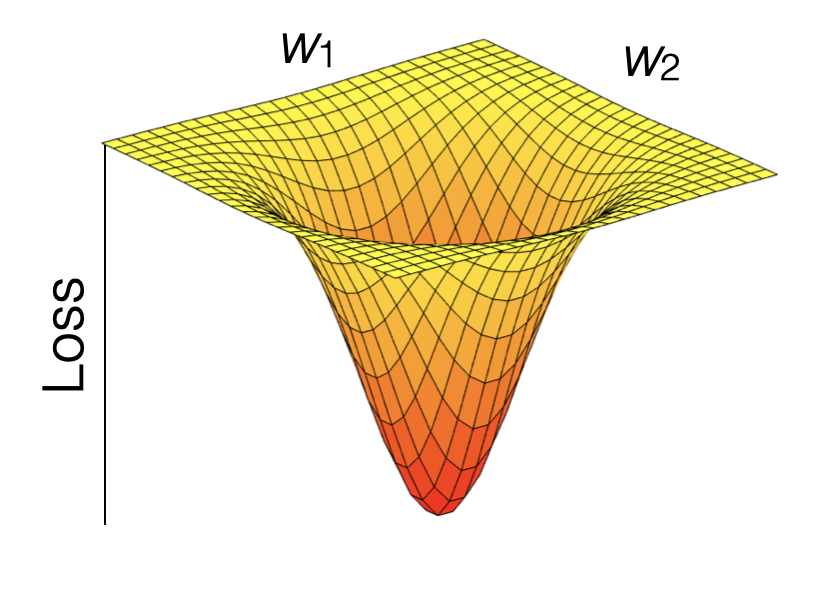
\includegraphics[width=11.5in]{./fig/loss_plane} 

}

\caption{Visualization of a loss function as a plane spanned by the two parameters $w_1$ and $w_2$.}\label{fig:unnamed-chunk-22}
\end{figure}

Model training is implemented in R for different algorithms in different packages. Some algorithms are even implemented by multiple packages (e.g., \texttt{nnet} and \texttt{neuralnet} for artificial neural networks). As described in Chapter \ref{preprocessing}, the \textbf{caret} package provides ``wrappers'' that handle a large selection of different ML model implementations in different packages with a unified interface (see \href{https://topepo.github.io/caret/available-models.html}{here} for an overview of available models). The \textbf{caret} function \texttt{train()} is the centre piece. Its argument \texttt{metric} specifies the loss function and defaults to the RMSE for regression models and accuracy for classification (see sub-section on metrics below).

\hypertarget{hyperparameter-tuning}{%
\section{Hyperparameter tuning}\label{hyperparameter-tuning}}

Practically all ML algorithms have some ``knobs'' to turn in order to achieve efficient model training and predictive performance. Such ``knobs'' are the \emph{hyperparameters}. What these knobs are, depends on the ML algorithm.

For KNN, this is \texttt{k} - the number of neighbours to consider for determining distances. There is always an optimum \(k\). Obviously, if \(k = n\), we consider all observations as neighbours and each prediction is simply the mean of all observed target values \(Y\), irrespective of the predictor values. This cannot be optimal and such a model is likely underfit. On the other extreme, with \(k = 1\), the model will be strongly affected by the noise in the single nearest neighbour and its generalisability will suffer. This should be reflected in a poor performance on the validation data.

For random forests from the \textbf{ranger} package, hyperparameters are:

\begin{itemize}
\tightlist
\item
  \texttt{mtry}: the number of variables to consider to make decisions, often taken as \(p/3\), where \(p\) is the number of predictors.
\item
  \texttt{min.node.size}: the number of data points at the ``bottom'' of each decision tree
\item
  \texttt{splitrule}: the function applied to data in each branch of a tree, used for determining the goodness of a decision
\end{itemize}

Hyperparameters usually have to be ``tuned''. The optimal setting depends on the data and can therefore not be known \emph{a priori}.

In \textbf{caret}, hyperparameter tuning is implemented as part of the \texttt{train()} function. Values of hyperparameters to consider are to be specified by the argument \texttt{tuneGrid}, which takes a data frame with column(s) named according to the name(s) of the hyperparameter(s) and rows for each combination of hyperparameters to consider.

\begin{Shaded}
\begin{Highlighting}[]
\DocumentationTok{\#\# do not run}
\FunctionTok{train}\NormalTok{(}
  \AttributeTok{form =}\NormalTok{ GPP\_NT\_VUT\_REF }\SpecialCharTok{\textasciitilde{}}\NormalTok{ SW\_F\_IN }\SpecialCharTok{+}\NormalTok{ VPD\_F }\SpecialCharTok{+}\NormalTok{ TA\_F, }
  \AttributeTok{data =}\NormalTok{ ddf, }
  \AttributeTok{method =} \StringTok{"ranger"}\NormalTok{,}
  \AttributeTok{tuneGrid =} \FunctionTok{expand.grid}\NormalTok{( }\AttributeTok{.mtry =} \FunctionTok{floor}\NormalTok{(}\DecValTok{6} \SpecialCharTok{/} \DecValTok{3}\NormalTok{),}
                          \AttributeTok{.min.node.size =} \FunctionTok{c}\NormalTok{(}\DecValTok{3}\NormalTok{, }\DecValTok{5}\NormalTok{, }\DecValTok{9}\NormalTok{,}\DecValTok{15}\NormalTok{, }\DecValTok{30}\NormalTok{),}
                          \AttributeTok{.splitrule =} \FunctionTok{c}\NormalTok{(}\StringTok{"variance"}\NormalTok{, }\StringTok{"maxstat"}\NormalTok{)),}
\NormalTok{  ...}
\NormalTok{)}
\end{Highlighting}
\end{Shaded}

Here, \texttt{expand.grid()} is used to provide a data frame with all combinations of values provided by individual vectors.

\hypertarget{resampling}{%
\section{Resampling}\label{resampling}}

The goal of model training is to achieve the best possible model generalisability. That is, the best possible model performance when predicting to data that was not used for training - the test data. Resampling mimicks the comparison of predictions to the test data. Instead of using all training data, the training data is \emph{resampled} into a number further splits into pairs of training and \emph{validation} data. Model training is then guided by minimising the average loss determined on each resample of the validation data. Having multiple resamples (multiple \emph{folds} of training-validation splits) avoids the loss minimization from being misguided by random peculiarities in the training and/or validation data.

A common resampling method is \emph{k-fold cross validation}, where the training data is split into \emph{k} equally sized subsets (\emph{folds}). Then, there will be \emph{k} iterations, where each fold is used for validation once (while the remaining folds are used for training). An extreme case is \emph{leave-one-out cross validation}, where \emph{k} corresponds to the number of data points.

\begin{center}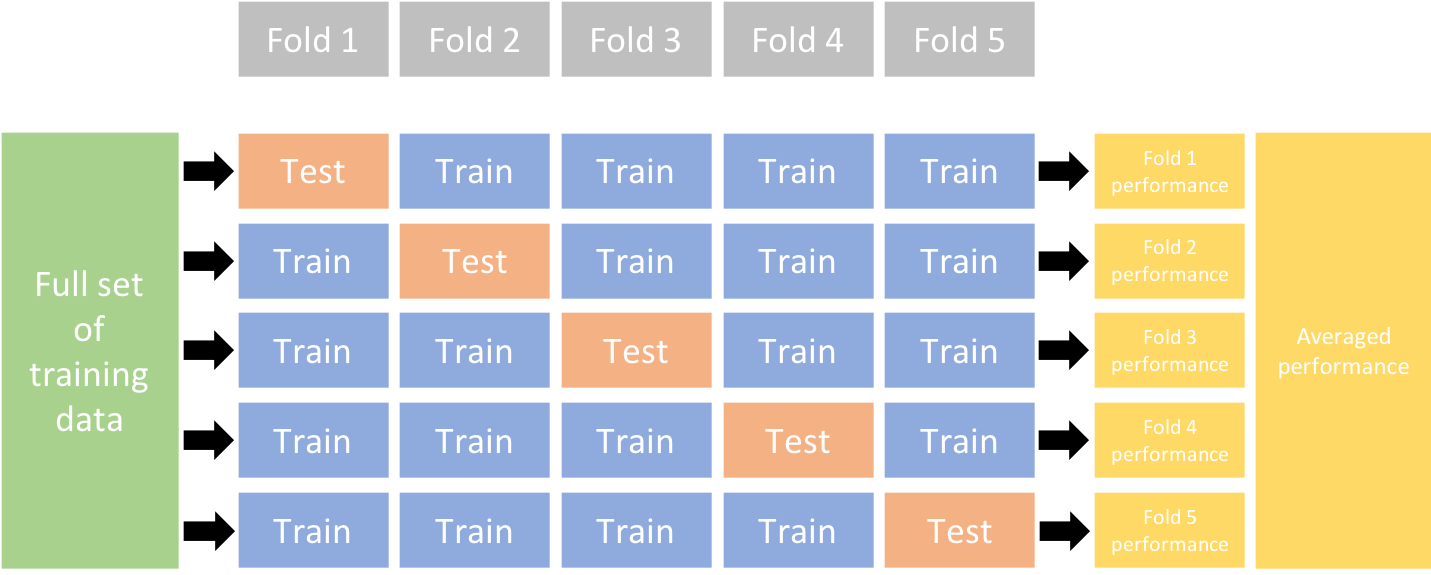
\includegraphics[width=19.88in]{fig/cv} \end{center}

To do a k-fold cross validation during model training in R, we don't have to implement the loops around folds ourselves. The resampling procedure can be specified in the \textbf{caret} function \texttt{train()} with the argument \texttt{trControl}. The object that this argument takes is the output of a function call to \texttt{trainControl()}. This can be implemented in two steps. For example, to do a 10-fold cross-validation, we can write:

\begin{Shaded}
\begin{Highlighting}[]
\DocumentationTok{\#\# do not run}
\FunctionTok{train}\NormalTok{(}
\NormalTok{  pp, }
  \AttributeTok{data =}\NormalTok{ ddf\_train, }
  \AttributeTok{method =} \StringTok{"ranger"}\NormalTok{,}
  \AttributeTok{tuneGrid =} \FunctionTok{expand.grid}\NormalTok{( }\AttributeTok{.mtry =} \FunctionTok{floor}\NormalTok{(}\DecValTok{6} \SpecialCharTok{/} \DecValTok{3}\NormalTok{),}
                          \AttributeTok{.min.node.size =} \FunctionTok{c}\NormalTok{(}\DecValTok{3}\NormalTok{, }\DecValTok{5}\NormalTok{, }\DecValTok{9}\NormalTok{,}\DecValTok{15}\NormalTok{, }\DecValTok{30}\NormalTok{),}
                          \AttributeTok{.splitrule =} \FunctionTok{c}\NormalTok{(}\StringTok{"variance"}\NormalTok{, }\StringTok{"maxstat"}\NormalTok{)),}
  \AttributeTok{trControl =} \FunctionTok{trainControl}\NormalTok{(}\AttributeTok{method =} \StringTok{"cv"}\NormalTok{, }\AttributeTok{number =} \DecValTok{10}\NormalTok{),}
\NormalTok{  ...}
\NormalTok{)}
\end{Highlighting}
\end{Shaded}

In certain cases, data points stem from different ``groups'', and generalisability across groups is critical. In such cases, data from a given group must not be used both in the training and validation sets. Instead, splits should be made along group delineations. The \emph{caret} function \texttt{groupKFold()} offers the solution for this case.

\hypertarget{exercises}{%
\chapter{Exercises}\label{exercises}}

Now that you are familiar with the basic steps for supervised machine learning, you can get your hands on the data yourself and implement code for addressing the modelling task outlined in Chapter \ref{motivation}.

\hypertarget{reading-and-cleaning}{%
\section{Reading and cleaning}\label{reading-and-cleaning}}

Read the CSV file \texttt{"./data/FLX\_CH-Dav\_FLUXNET2015\_FULLSET\_DD\_1997-2014\_1-3.csv"}, select all variables with name ending with \texttt{"\_F"}, the variables \texttt{"TIMESTAMP"}, \texttt{"GPP\_NT\_VUT\_REF"}, and \texttt{"NEE\_VUT\_REF\_QC"}, and drop all variables that contain \texttt{"JSB"} in their name. Then convert the variable \texttt{"TIMESTAMP"} to a date-time object with the function \texttt{ymd()} from the \emph{lubridate} package, and interpret all values \texttt{-9999} as missing values. Then, set all values of \texttt{"GPP\_NT\_VUT\_REF"} to missing if the corresponding quality control variable indicates that less than 90\% are measured data points. Finally, drop the variable \texttt{"NEE\_VUT\_REF\_QC"} - we won't use it anymore.

\begin{Shaded}
\begin{Highlighting}[]
\DocumentationTok{\#\# write your code here}
\end{Highlighting}
\end{Shaded}

\hypertarget{data-splitting-1}{%
\section{Data splitting}\label{data-splitting-1}}

Split the data a training and testing set, that contain 70\% and 30\% of the total available data, respectively.

\begin{Shaded}
\begin{Highlighting}[]
\DocumentationTok{\#\# write your code here}
\end{Highlighting}
\end{Shaded}

\hypertarget{linear-model}{%
\section{Linear model}\label{linear-model}}

\hypertarget{training-1}{%
\subsection{Training}\label{training-1}}

Fit a linear regression model using the base-R function \texttt{lm()} and the training set. The target variable is \texttt{"GPP\_NT\_VUT\_REF"}, and predictor variables are all available meterological variables in the dataset. Answer the following questions:

\begin{itemize}
\tightlist
\item
  What is the \(R^2\) of predicted vs.~observed \texttt{"GPP\_NT\_VUT\_REF"}?
\item
  Is the linear regression slope significantly different from zero for all predictors?
\item
  Is a linear regression model with ``poor'' predictors removed better supported by the data than a model including all predictors?
\end{itemize}

\begin{Shaded}
\begin{Highlighting}[]
\DocumentationTok{\#\# write your code here}
\end{Highlighting}
\end{Shaded}

Use caret and the function \texttt{train()} for fitting the same linear regression model (with all predictors) on the same data. Does it yield identical results as using \texttt{lm()} directly? You will have to set the argument \texttt{trControl} accordingly to avoid resampling, and instead fit the model on the all data in \texttt{ddf\_train}. You can use \texttt{summary()} also on the object returned by the function \texttt{train()}.

\begin{Shaded}
\begin{Highlighting}[]
\DocumentationTok{\#\# write your code here}
\end{Highlighting}
\end{Shaded}

\hypertarget{prediction}{%
\subsection{Prediction}\label{prediction}}

With the model containing all predictors and fitted on \texttt{ddf\_train}, make predictions using first \texttt{ddf\_train} and then \texttt{ddf\_test}. Compute the \(R^2\) and the root-mean-square error, and visualise modelled vs.~observed values to evaluate both predictions.

Do you expect the linear regression model trained on \texttt{ddf\_train} to predict substantially better on \texttt{ddf\_train} than on \texttt{ddf\_test}? Why (not)?

Hints:

\begin{itemize}
\tightlist
\item
  To calculate predictions, use the generic function \texttt{predict()} with the argument \texttt{newdata\ =\ ...}.
\item
  The \(R^2\) can be extracted from the model object as \texttt{summary(model\_object)\$r.squared}, or is (as the RMSE) given in the metrics data frame returned by \texttt{metrics()} from the \emph{yardstick} library.
\item
  For visualisation the model performance, consider a scatterplot, or (better) a plot that reveals the density of overlapping points. (We're plotting information from over 4000 data points here!)
\end{itemize}

\begin{Shaded}
\begin{Highlighting}[]
\DocumentationTok{\#\# write your code here}
\end{Highlighting}
\end{Shaded}

\hypertarget{knn}{%
\section{KNN}\label{knn}}

\hypertarget{check-data}{%
\subsection{Check data}\label{check-data}}

\begin{Shaded}
\begin{Highlighting}[]
\DocumentationTok{\#\# write your code here}
\end{Highlighting}
\end{Shaded}

The variable \texttt{PA\_F} looks weird and was not significant in the linear model. Therefore, we won't use it for the models below.

\hypertarget{training-2}{%
\subsection{Training}\label{training-2}}

Fit two KNN models on \texttt{ddf\_train} (excluding \texttt{"PA\_F"}), one with \(k = 2\) and one with \(k = 30\), both without resampling. Use the RMSE as the loss function. Center and scale data as part of the pre-processing and model formulation specification using the function \texttt{recipe()}.

\begin{Shaded}
\begin{Highlighting}[]
\DocumentationTok{\#\# write your code here}
\end{Highlighting}
\end{Shaded}

\hypertarget{prediction-1}{%
\subsection{Prediction}\label{prediction-1}}

With the two models fitted above, predict \texttt{"GPP\_NT\_VUT\_REF"} for both and training and the testing sets, and evaluate them as above (metrics and visualisation).

Which model do you expect to perform better on the training set and which to perform better on the testing set? Why? Do you find evidence for overfitting in any of the models?

\begin{Shaded}
\begin{Highlighting}[]
\DocumentationTok{\#\# write your code here}
\end{Highlighting}
\end{Shaded}

\hypertarget{sample-hyperparameters}{%
\subsection{Sample hyperparameters}\label{sample-hyperparameters}}

Train a KNN model with hyperparameter (\(k\)) tuned, and with five-fold cross validation, using the training set. As the loss function, use RMSE. Sample the following values for \(k\): 2, 5, 10, 15, 18, 20, 22, 24, 26, 30, 35, 40, 60, 100. Visualise the RMSE as a function of \(k\).

Hint:

\begin{itemize}
\tightlist
\item
  The visualisation of cross-validation results can be visualised with the \texttt{plot(model\_object)} of \texttt{ggplot(model\_object)}.
\end{itemize}

\begin{Shaded}
\begin{Highlighting}[]
\DocumentationTok{\#\# write your code here}
\end{Highlighting}
\end{Shaded}

\hypertarget{random-forest-1}{%
\section{Random forest}\label{random-forest-1}}

\hypertarget{training-3}{%
\subsection{Training}\label{training-3}}

Fit a random forest model with \texttt{ddf\_train} and all predictors excluding \texttt{"PA\_F"} and five-fold cross validation. Use RMSE as the loss function.

Hints:

\begin{itemize}
\tightlist
\item
  Use the package \emph{ranger} which implements the random forest algorithm.
\item
  See \href{https://topepo.github.io/caret/available-models.html}{here} for information about hyperparameters available for tuning with caret.
\item
  Set the argument \texttt{savePredictions\ =\ "final"} of function \texttt{trainControl()}.
\end{itemize}

\begin{Shaded}
\begin{Highlighting}[]
\DocumentationTok{\#\# write your code here}
\end{Highlighting}
\end{Shaded}

\hypertarget{prediction-2}{%
\subsection{Prediction}\label{prediction-2}}

Evaluate the trained model on the training and on the test set, giving metrics and a visualisation as above.

How are differences in performance to be interpreted? Compare the performances of linear regression, KNN, and random forest, considering the evaluation on the test set.

\begin{Shaded}
\begin{Highlighting}[]
\DocumentationTok{\#\# write your code here}
\end{Highlighting}
\end{Shaded}

Show the model performance (metrics and visualisation) on the validation sets all cross validation folds combined.

Do you expect it to be more similar to the model performance on the training set or the testing set in the evaluation above? Why?

\begin{Shaded}
\begin{Highlighting}[]
\DocumentationTok{\#\# write your code here}
\end{Highlighting}
\end{Shaded}

\hypertarget{solutions}{%
\chapter{Solutions}\label{solutions}}

Now that you are familiar with the basic steps for supervised machine learning, you can get your hands on the data yourself and implement code for addressing the modelling task outlined in Chapter \ref{motivation}.

\hypertarget{reading-and-cleaning-1}{%
\section{Reading and cleaning}\label{reading-and-cleaning-1}}

Read the CSV file \texttt{"./data/FLX\_CH-Dav\_FLUXNET2015\_FULLSET\_DD\_1997-2014\_1-3.csv"}, select all variables with name ending with \texttt{"\_F"}, the variables \texttt{"TIMESTAMP"}, \texttt{"GPP\_NT\_VUT\_REF"}, and \texttt{"NEE\_VUT\_REF\_QC"}, and drop all variables that contain \texttt{"JSB"} in their name. Then convert the variable \texttt{"TIMESTAMP"} to a date-time object with the function \texttt{ymd()} from the \emph{lubridate} package, and interpret all values \texttt{-9999} as missing values. Then, set all values of \texttt{"GPP\_NT\_VUT\_REF"} to missing if the corresponding quality control variable indicates that less than 90\% are measured data points. Finally, drop the variable \texttt{"NEE\_VUT\_REF\_QC"} - we won't use it anymore.

\begin{Shaded}
\begin{Highlighting}[]
\FunctionTok{library}\NormalTok{(tidyverse)}

\NormalTok{ddf }\OtherTok{\textless{}{-}} \FunctionTok{read\_csv}\NormalTok{(}\StringTok{"./data/FLX\_CH{-}Dav\_FLUXNET2015\_FULLSET\_DD\_1997{-}2014\_1{-}3.csv"}\NormalTok{) }\SpecialCharTok{\%\textgreater{}\%} 
  
  \DocumentationTok{\#\# select only the variables we are interested in}
  \FunctionTok{select}\NormalTok{(}\FunctionTok{starts\_with}\NormalTok{(}\StringTok{"TIMESTAMP"}\NormalTok{),}
         \FunctionTok{ends\_with}\NormalTok{(}\StringTok{"\_F"}\NormalTok{),   }\CommentTok{\# all meteorological variables}
\NormalTok{         GPP\_NT\_VUT\_REF,}
\NormalTok{         NEE\_VUT\_REF\_QC,}
         \SpecialCharTok{{-}}\FunctionTok{contains}\NormalTok{(}\StringTok{"JSB"}\NormalTok{)) }\SpecialCharTok{\%\textgreater{}\%}

  \DocumentationTok{\#\# convert to a nice date object}
  \FunctionTok{mutate}\NormalTok{(}\AttributeTok{TIMESTAMP =}\NormalTok{ lubridate}\SpecialCharTok{::}\FunctionTok{ymd}\NormalTok{(TIMESTAMP)) }\SpecialCharTok{\%\textgreater{}\%}

  \DocumentationTok{\#\# set all {-}9999 to NA}
  \FunctionTok{na\_if}\NormalTok{(}\SpecialCharTok{{-}}\DecValTok{9999}\NormalTok{) }\SpecialCharTok{\%\textgreater{}\%}

  \DocumentationTok{\#\# drop QC variables (no longer needed), except NEE\_VUT\_REF\_QC}
  \FunctionTok{select}\NormalTok{(}\SpecialCharTok{{-}}\FunctionTok{ends\_with}\NormalTok{(}\StringTok{"\_QC"}\NormalTok{), NEE\_VUT\_REF\_QC) }\SpecialCharTok{\%\textgreater{}\%} 

  \FunctionTok{mutate}\NormalTok{(}\AttributeTok{GPP\_NT\_VUT\_REF =} \FunctionTok{ifelse}\NormalTok{(NEE\_VUT\_REF\_QC }\SpecialCharTok{\textless{}} \FloatTok{0.9}\NormalTok{, }\ConstantTok{NA}\NormalTok{, GPP\_NT\_VUT\_REF)) }\SpecialCharTok{\%\textgreater{}\%} 
  \FunctionTok{select}\NormalTok{(}\SpecialCharTok{{-}}\NormalTok{NEE\_VUT\_REF\_QC)}
\end{Highlighting}
\end{Shaded}

\hypertarget{data-splitting-2}{%
\section{Data splitting}\label{data-splitting-2}}

Split the data a training and testing set, that contain 70\% and 30\% of the total available data, respectively.

\begin{Shaded}
\begin{Highlighting}[]
\FunctionTok{library}\NormalTok{(rsample)}
\FunctionTok{set.seed}\NormalTok{(}\DecValTok{1982}\NormalTok{)  }\CommentTok{\# for reproducibility}
\NormalTok{split }\OtherTok{\textless{}{-}} \FunctionTok{initial\_split}\NormalTok{(ddf, }\AttributeTok{prop =} \FloatTok{0.7}\NormalTok{)}
\NormalTok{ddf\_train }\OtherTok{\textless{}{-}} \FunctionTok{training}\NormalTok{(split)}
\NormalTok{ddf\_test }\OtherTok{\textless{}{-}} \FunctionTok{testing}\NormalTok{(split)}
\end{Highlighting}
\end{Shaded}

\hypertarget{linear-model-1}{%
\section{Linear model}\label{linear-model-1}}

\hypertarget{training-4}{%
\subsection{Training}\label{training-4}}

Fit a linear regression model using the base-R function \texttt{lm()} and the training set. The target variable is \texttt{"GPP\_NT\_VUT\_REF"}, and predictor variables are all available meterological variables in the dataset. Answer the following questions:

\begin{itemize}
\tightlist
\item
  What is the \(R^2\) of predicted vs.~observed \texttt{"GPP\_NT\_VUT\_REF"}?
\item
  Is the linear regression slope significantly different from zero for all predictors?
\item
  Is a linear regression model with ``poor'' predictors removed better supported by the data than a model including all predictors?
\end{itemize}

\begin{Shaded}
\begin{Highlighting}[]
\DocumentationTok{\#\# fit linear regression model}
\NormalTok{linmod\_baser }\OtherTok{\textless{}{-}} \FunctionTok{lm}\NormalTok{(}
  \AttributeTok{form =}\NormalTok{ GPP\_NT\_VUT\_REF }\SpecialCharTok{\textasciitilde{}}\NormalTok{ ., }
  \AttributeTok{data =}\NormalTok{ ddf\_train }\SpecialCharTok{\%\textgreater{}\%} 
    \FunctionTok{drop\_na}\NormalTok{() }\SpecialCharTok{\%\textgreater{}\%} 
    \FunctionTok{select}\NormalTok{(}\SpecialCharTok{{-}}\NormalTok{TIMESTAMP)}
\NormalTok{)}

\DocumentationTok{\#\# show summary information of the model}
\FunctionTok{summary}\NormalTok{(linmod\_baser)}
\end{Highlighting}
\end{Shaded}

\begin{verbatim}
## 
## Call:
## lm(formula = GPP_NT_VUT_REF ~ ., data = ddf_train %>% drop_na() %>% 
##     select(-TIMESTAMP))
## 
## Residuals:
##     Min      1Q  Median      3Q     Max 
## -5.1941 -1.0393 -0.1299  0.8859  7.7205 
## 
## Coefficients:
##               Estimate Std. Error t value Pr(>|t|)    
## (Intercept) -0.9570704  3.4840107  -0.275 0.783558    
## TA_F         0.1633211  0.0108181  15.097  < 2e-16 ***
## SW_IN_F      0.0137226  0.0003914  35.064  < 2e-16 ***
## LW_IN_F      0.0207311  0.0012040  17.219  < 2e-16 ***
## VPD_F       -0.1420886  0.0195509  -7.268 4.35e-13 ***
## PA_F        -0.0402727  0.0404675  -0.995 0.319704    
## P_F         -0.0214314  0.0046177  -4.641 3.57e-06 ***
## WS_F        -0.1418356  0.0398616  -3.558 0.000378 ***
## ---
## Signif. codes:  0 '***' 0.001 '**' 0.01 '*' 0.05 '.' 0.1 ' ' 1
## 
## Residual standard error: 1.549 on 4135 degrees of freedom
## Multiple R-squared:  0.6904, Adjusted R-squared:  0.6899 
## F-statistic:  1317 on 7 and 4135 DF,  p-value: < 2.2e-16
\end{verbatim}

\begin{Shaded}
\begin{Highlighting}[]
\DocumentationTok{\#\# Models can be compared, for example by the Bayesian Information Criterion (BIC). }
\DocumentationTok{\#\# It penalizes complex models and is optimal (lowest) where the trade{-}off between }
\DocumentationTok{\#\# explanatory power on the training set vs. number of predictors is best. The BIC}
\DocumentationTok{\#\# tends to be more conservative than the AIC.}
\FunctionTok{BIC}\NormalTok{(linmod\_baser)}
\end{Highlighting}
\end{Shaded}

\begin{verbatim}
## [1] 15450.89
\end{verbatim}

\begin{Shaded}
\begin{Highlighting}[]
\DocumentationTok{\#\# Fit an lm model on the same data, but with PA\_F removed.}
\NormalTok{linmod\_baser\_nopaf }\OtherTok{\textless{}{-}} \FunctionTok{lm}\NormalTok{(}
  \AttributeTok{form =}\NormalTok{ GPP\_NT\_VUT\_REF }\SpecialCharTok{\textasciitilde{}}\NormalTok{ ., }
  \AttributeTok{data =}\NormalTok{ ddf\_train }\SpecialCharTok{\%\textgreater{}\%} 
    \FunctionTok{drop\_na}\NormalTok{() }\SpecialCharTok{\%\textgreater{}\%} 
    \FunctionTok{select}\NormalTok{(}\SpecialCharTok{{-}}\NormalTok{TIMESTAMP, }\SpecialCharTok{{-}}\NormalTok{PA\_F)}
\NormalTok{)}

\DocumentationTok{\#\# The R{-}squared is slightly lower here (0.6903) than in the model with all predictors (0.6904)}
\FunctionTok{summary}\NormalTok{(linmod\_baser\_nopaf)}
\end{Highlighting}
\end{Shaded}

\begin{verbatim}
## 
## Call:
## lm(formula = GPP_NT_VUT_REF ~ ., data = ddf_train %>% drop_na() %>% 
##     select(-TIMESTAMP, -PA_F))
## 
## Residuals:
##     Min      1Q  Median      3Q     Max 
## -5.1849 -1.0390 -0.1306  0.8867  7.7594 
## 
## Coefficients:
##               Estimate Std. Error t value Pr(>|t|)    
## (Intercept) -4.4102425  0.3135013 -14.068  < 2e-16 ***
## TA_F         0.1595814  0.0101445  15.731  < 2e-16 ***
## SW_IN_F      0.0136923  0.0003902  35.093  < 2e-16 ***
## LW_IN_F      0.0210424  0.0011626  18.099  < 2e-16 ***
## VPD_F       -0.1400240  0.0194405  -7.203 6.98e-13 ***
## P_F         -0.0212661  0.0046147  -4.608 4.18e-06 ***
## WS_F        -0.1343263  0.0391409  -3.432 0.000605 ***
## ---
## Signif. codes:  0 '***' 0.001 '**' 0.01 '*' 0.05 '.' 0.1 ' ' 1
## 
## Residual standard error: 1.549 on 4136 degrees of freedom
## Multiple R-squared:  0.6903, Adjusted R-squared:  0.6899 
## F-statistic:  1537 on 6 and 4136 DF,  p-value: < 2.2e-16
\end{verbatim}

\begin{Shaded}
\begin{Highlighting}[]
\DocumentationTok{\#\# ... but the BIC is clearly lower, indicating that the model with PA\_F removed is better.}
\FunctionTok{BIC}\NormalTok{(linmod\_baser\_nopaf)}
\end{Highlighting}
\end{Shaded}

\begin{verbatim}
## [1] 15443.55
\end{verbatim}

Use caret and the function \texttt{train()} for fitting the same linear regression model (with all predictors) on the same data. Does it yield identical results as using \texttt{lm()} directly? You will have to set the argument \texttt{trControl} accordingly to avoid resampling, and instead fit the model on the all data in \texttt{ddf\_train}. You can use \texttt{summary()} also on the object returned by the function \texttt{train()}.

\begin{Shaded}
\begin{Highlighting}[]
\FunctionTok{library}\NormalTok{(caret)}

\NormalTok{linmod\_caret }\OtherTok{\textless{}{-}} \FunctionTok{train}\NormalTok{(}
  \AttributeTok{form =}\NormalTok{ GPP\_NT\_VUT\_REF }\SpecialCharTok{\textasciitilde{}}\NormalTok{ ., }
  \AttributeTok{data =}\NormalTok{ ddf\_train }\SpecialCharTok{\%\textgreater{}\%} 
    \FunctionTok{drop\_na}\NormalTok{() }\SpecialCharTok{\%\textgreater{}\%} 
    \FunctionTok{select}\NormalTok{(}\SpecialCharTok{{-}}\NormalTok{TIMESTAMP), }
  \AttributeTok{method =} \StringTok{"lm"}\NormalTok{,}
  \AttributeTok{trControl =} \FunctionTok{trainControl}\NormalTok{(}\AttributeTok{method =} \StringTok{"none"}\NormalTok{)}
\NormalTok{)}

\FunctionTok{summary}\NormalTok{(linmod\_caret)}
\end{Highlighting}
\end{Shaded}

\begin{verbatim}
## 
## Call:
## lm(formula = .outcome ~ ., data = dat)
## 
## Residuals:
##     Min      1Q  Median      3Q     Max 
## -5.1941 -1.0393 -0.1299  0.8859  7.7205 
## 
## Coefficients:
##               Estimate Std. Error t value Pr(>|t|)    
## (Intercept) -0.9570704  3.4840107  -0.275 0.783558    
## TA_F         0.1633211  0.0108181  15.097  < 2e-16 ***
## SW_IN_F      0.0137226  0.0003914  35.064  < 2e-16 ***
## LW_IN_F      0.0207311  0.0012040  17.219  < 2e-16 ***
## VPD_F       -0.1420886  0.0195509  -7.268 4.35e-13 ***
## PA_F        -0.0402727  0.0404675  -0.995 0.319704    
## P_F         -0.0214314  0.0046177  -4.641 3.57e-06 ***
## WS_F        -0.1418356  0.0398616  -3.558 0.000378 ***
## ---
## Signif. codes:  0 '***' 0.001 '**' 0.01 '*' 0.05 '.' 0.1 ' ' 1
## 
## Residual standard error: 1.549 on 4135 degrees of freedom
## Multiple R-squared:  0.6904, Adjusted R-squared:  0.6899 
## F-statistic:  1317 on 7 and 4135 DF,  p-value: < 2.2e-16
\end{verbatim}

\hypertarget{prediction-3}{%
\subsection{Prediction}\label{prediction-3}}

With the model containing all predictors and fitted on \texttt{ddf\_train}, make predictions using first \texttt{ddf\_train} and then \texttt{ddf\_test}. Compute the \(R^2\) and the root-mean-square error, and visualise modelled vs.~observed values to evaluate both predictions.

Do you expect the linear regression model trained on \texttt{ddf\_train} to predict substantially better on \texttt{ddf\_train} than on \texttt{ddf\_test}? Why (not)?

Hints:

\begin{itemize}
\tightlist
\item
  To calculate predictions, use the generic function \texttt{predict()} with the argument \texttt{newdata\ =\ ...}.
\item
  The \(R^2\) can be extracted from the model object as \texttt{summary(model\_object)\$r.squared}, or is (as the RMSE) given in the metrics data frame returned by \texttt{metrics()} from the \emph{yardstick} library.
\item
  For visualisation the model performance, consider a scatterplot, or (better) a plot that reveals the density of overlapping points. (We're plotting information from over 4000 data points here!)
\end{itemize}

\begin{Shaded}
\begin{Highlighting}[]
\FunctionTok{library}\NormalTok{(patchwork)}
\FunctionTok{library}\NormalTok{(yardstick)}

\DocumentationTok{\#\# made into a function to reuse code below}
\NormalTok{eval\_model }\OtherTok{\textless{}{-}} \ControlFlowTok{function}\NormalTok{(mod, df\_train, df\_test)\{}
  
  \DocumentationTok{\#\# add predictions to the data frames}
\NormalTok{  df\_train }\OtherTok{\textless{}{-}}\NormalTok{ df\_train }\SpecialCharTok{\%\textgreater{}\%} 
    \FunctionTok{drop\_na}\NormalTok{() }\SpecialCharTok{\%\textgreater{}\%} 
    \FunctionTok{mutate}\NormalTok{(}\AttributeTok{fitted =}  \FunctionTok{predict}\NormalTok{(mod, }\AttributeTok{newdata =}\NormalTok{ .))}
  
\NormalTok{  df\_test }\OtherTok{\textless{}{-}}\NormalTok{ df\_test }\SpecialCharTok{\%\textgreater{}\%} 
    \FunctionTok{drop\_na}\NormalTok{() }\SpecialCharTok{\%\textgreater{}\%} 
    \FunctionTok{mutate}\NormalTok{(}\AttributeTok{fitted =}  \FunctionTok{predict}\NormalTok{(mod, }\AttributeTok{newdata =}\NormalTok{ .))}
  
  \DocumentationTok{\#\# get metrics tables}
\NormalTok{  metrics\_train }\OtherTok{\textless{}{-}}\NormalTok{ df\_train }\SpecialCharTok{\%\textgreater{}\%} 
\NormalTok{    yardstick}\SpecialCharTok{::}\FunctionTok{metrics}\NormalTok{(GPP\_NT\_VUT\_REF, fitted)}
  
\NormalTok{  metrics\_test }\OtherTok{\textless{}{-}}\NormalTok{ df\_test }\SpecialCharTok{\%\textgreater{}\%} 
\NormalTok{    yardstick}\SpecialCharTok{::}\FunctionTok{metrics}\NormalTok{(GPP\_NT\_VUT\_REF, fitted)}
  
  \DocumentationTok{\#\# extract values from metrics tables}
\NormalTok{  rmse\_train }\OtherTok{\textless{}{-}}\NormalTok{ metrics\_train }\SpecialCharTok{\%\textgreater{}\%} 
    \FunctionTok{filter}\NormalTok{(.metric }\SpecialCharTok{==} \StringTok{"rmse"}\NormalTok{) }\SpecialCharTok{\%\textgreater{}\%} 
    \FunctionTok{pull}\NormalTok{(.estimate)}
\NormalTok{  rsq\_train }\OtherTok{\textless{}{-}}\NormalTok{ metrics\_train }\SpecialCharTok{\%\textgreater{}\%} 
    \FunctionTok{filter}\NormalTok{(.metric }\SpecialCharTok{==} \StringTok{"rsq"}\NormalTok{) }\SpecialCharTok{\%\textgreater{}\%} 
    \FunctionTok{pull}\NormalTok{(.estimate)}
  
\NormalTok{  rmse\_test }\OtherTok{\textless{}{-}}\NormalTok{ metrics\_test }\SpecialCharTok{\%\textgreater{}\%} 
    \FunctionTok{filter}\NormalTok{(.metric }\SpecialCharTok{==} \StringTok{"rmse"}\NormalTok{) }\SpecialCharTok{\%\textgreater{}\%} 
    \FunctionTok{pull}\NormalTok{(.estimate)}
\NormalTok{  rsq\_test }\OtherTok{\textless{}{-}}\NormalTok{ metrics\_test }\SpecialCharTok{\%\textgreater{}\%} 
    \FunctionTok{filter}\NormalTok{(.metric }\SpecialCharTok{==} \StringTok{"rsq"}\NormalTok{) }\SpecialCharTok{\%\textgreater{}\%} 
    \FunctionTok{pull}\NormalTok{(.estimate)}
  
  \DocumentationTok{\#\# visualise with a hexagon binning and a customised color scale,}
  \DocumentationTok{\#\# adding information of metrics as sub{-}titles}
\NormalTok{  gg1 }\OtherTok{\textless{}{-}}\NormalTok{ df\_train }\SpecialCharTok{\%\textgreater{}\%} 
    \FunctionTok{ggplot}\NormalTok{(}\FunctionTok{aes}\NormalTok{(GPP\_NT\_VUT\_REF, fitted)) }\SpecialCharTok{+}
    \FunctionTok{geom\_hex}\NormalTok{() }\SpecialCharTok{+}
    \FunctionTok{scale\_fill\_gradientn}\NormalTok{(}
      \AttributeTok{colours =} \FunctionTok{colorRampPalette}\NormalTok{( }\FunctionTok{c}\NormalTok{(}\StringTok{"gray65"}\NormalTok{, }\StringTok{"navy"}\NormalTok{, }\StringTok{"red"}\NormalTok{, }\StringTok{"yellow"}\NormalTok{))(}\DecValTok{5}\NormalTok{)) }\SpecialCharTok{+}
    \FunctionTok{geom\_abline}\NormalTok{(}\AttributeTok{slope =} \DecValTok{1}\NormalTok{, }\AttributeTok{intercept =} \DecValTok{0}\NormalTok{, }\AttributeTok{linetype =} \StringTok{"dotted"}\NormalTok{) }\SpecialCharTok{+}
    \FunctionTok{labs}\NormalTok{(}\AttributeTok{subtitle =} \FunctionTok{bquote}\NormalTok{( }\FunctionTok{italic}\NormalTok{(R)}\SpecialCharTok{\^{}}\DecValTok{2} \SpecialCharTok{==}\NormalTok{ .(}\FunctionTok{format}\NormalTok{(rsq\_train, }\AttributeTok{digits =} \DecValTok{2}\NormalTok{)) }\SpecialCharTok{\textasciitilde{}}\ErrorTok{\textasciitilde{}}
\NormalTok{                            RMSE }\SpecialCharTok{==}\NormalTok{ .(}\FunctionTok{format}\NormalTok{(rmse\_train, }\AttributeTok{digits =} \DecValTok{3}\NormalTok{))),}
         \AttributeTok{title =} \StringTok{"Training set"}\NormalTok{) }\SpecialCharTok{+}
    \FunctionTok{theme\_classic}\NormalTok{()}
  
\NormalTok{  gg2 }\OtherTok{\textless{}{-}}\NormalTok{ df\_test }\SpecialCharTok{\%\textgreater{}\%} 
    \FunctionTok{ggplot}\NormalTok{(}\FunctionTok{aes}\NormalTok{(GPP\_NT\_VUT\_REF, fitted)) }\SpecialCharTok{+}
    \FunctionTok{geom\_hex}\NormalTok{() }\SpecialCharTok{+}
    \FunctionTok{scale\_fill\_gradientn}\NormalTok{(}
      \AttributeTok{colours =} \FunctionTok{colorRampPalette}\NormalTok{( }\FunctionTok{c}\NormalTok{(}\StringTok{"gray65"}\NormalTok{, }\StringTok{"navy"}\NormalTok{, }\StringTok{"red"}\NormalTok{, }\StringTok{"yellow"}\NormalTok{))(}\DecValTok{5}\NormalTok{)) }\SpecialCharTok{+}
    \FunctionTok{geom\_abline}\NormalTok{(}\AttributeTok{slope =} \DecValTok{1}\NormalTok{, }\AttributeTok{intercept =} \DecValTok{0}\NormalTok{, }\AttributeTok{linetype =} \StringTok{"dotted"}\NormalTok{) }\SpecialCharTok{+}
    \FunctionTok{labs}\NormalTok{(}\AttributeTok{subtitle =} \FunctionTok{bquote}\NormalTok{( }\FunctionTok{italic}\NormalTok{(R)}\SpecialCharTok{\^{}}\DecValTok{2} \SpecialCharTok{==}\NormalTok{ .(}\FunctionTok{format}\NormalTok{(rsq\_test, }\AttributeTok{digits =} \DecValTok{2}\NormalTok{)) }\SpecialCharTok{\textasciitilde{}}\ErrorTok{\textasciitilde{}}
\NormalTok{                            RMSE }\SpecialCharTok{==}\NormalTok{ .(}\FunctionTok{format}\NormalTok{(rmse\_test, }\AttributeTok{digits =} \DecValTok{3}\NormalTok{))),}
         \AttributeTok{title =} \StringTok{"Test set"}\NormalTok{) }\SpecialCharTok{+}
    \FunctionTok{theme\_classic}\NormalTok{()}
  
  \FunctionTok{return}\NormalTok{(gg1 }\SpecialCharTok{+}\NormalTok{ gg2)}
\NormalTok{\}}

\FunctionTok{eval\_model}\NormalTok{(}\AttributeTok{mod =}\NormalTok{ linmod\_baser, }\AttributeTok{df\_train =}\NormalTok{ ddf\_train, }\AttributeTok{df\_test =}\NormalTok{ ddf\_test)}
\end{Highlighting}
\end{Shaded}

\begin{center}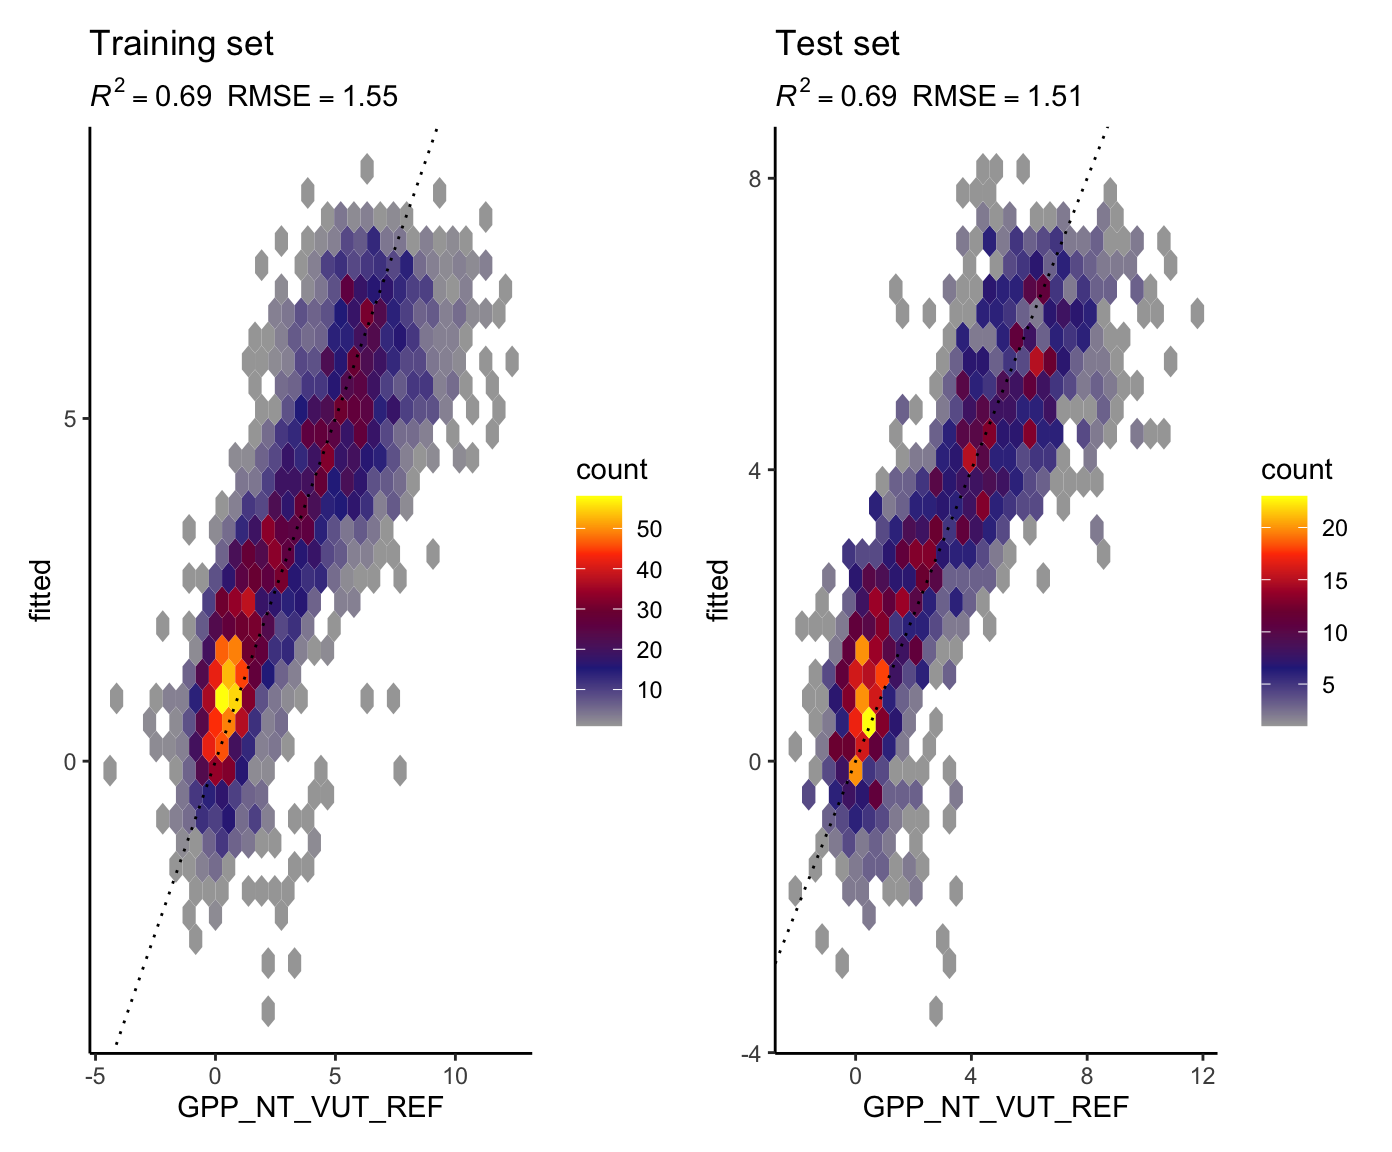
\includegraphics{ml4ec_workshop_files/figure-latex/unnamed-chunk-43-1} \end{center}

\hypertarget{knn-1}{%
\section{KNN}\label{knn-1}}

\hypertarget{check-data-1}{%
\subsection{Check data}\label{check-data-1}}

\begin{Shaded}
\begin{Highlighting}[]
\NormalTok{ddf\_train }\SpecialCharTok{\%\textgreater{}\%} 
  \FunctionTok{mutate}\NormalTok{(}\AttributeTok{split =} \StringTok{"train"}\NormalTok{) }\SpecialCharTok{\%\textgreater{}\%} 
  \FunctionTok{bind\_rows}\NormalTok{(ddf\_test }\SpecialCharTok{\%\textgreater{}\%} 
    \FunctionTok{mutate}\NormalTok{(}\AttributeTok{split =} \StringTok{"test"}\NormalTok{)) }\SpecialCharTok{\%\textgreater{}\%} 
  \FunctionTok{pivot\_longer}\NormalTok{(}\AttributeTok{cols =} \DecValTok{2}\SpecialCharTok{:}\DecValTok{9}\NormalTok{, }\AttributeTok{names\_to =} \StringTok{"variable"}\NormalTok{, }\AttributeTok{values\_to =} \StringTok{"value"}\NormalTok{) }\SpecialCharTok{\%\textgreater{}\%} 
  \FunctionTok{ggplot}\NormalTok{(}\FunctionTok{aes}\NormalTok{(}\AttributeTok{x =}\NormalTok{ value, }\AttributeTok{y =}\NormalTok{ ..density.., }\AttributeTok{color =}\NormalTok{ split)) }\SpecialCharTok{+}
  \FunctionTok{geom\_density}\NormalTok{() }\SpecialCharTok{+}
  \FunctionTok{facet\_wrap}\NormalTok{(}\SpecialCharTok{\textasciitilde{}}\NormalTok{variable, }\AttributeTok{scales =} \StringTok{"free"}\NormalTok{)}
\end{Highlighting}
\end{Shaded}

\begin{center}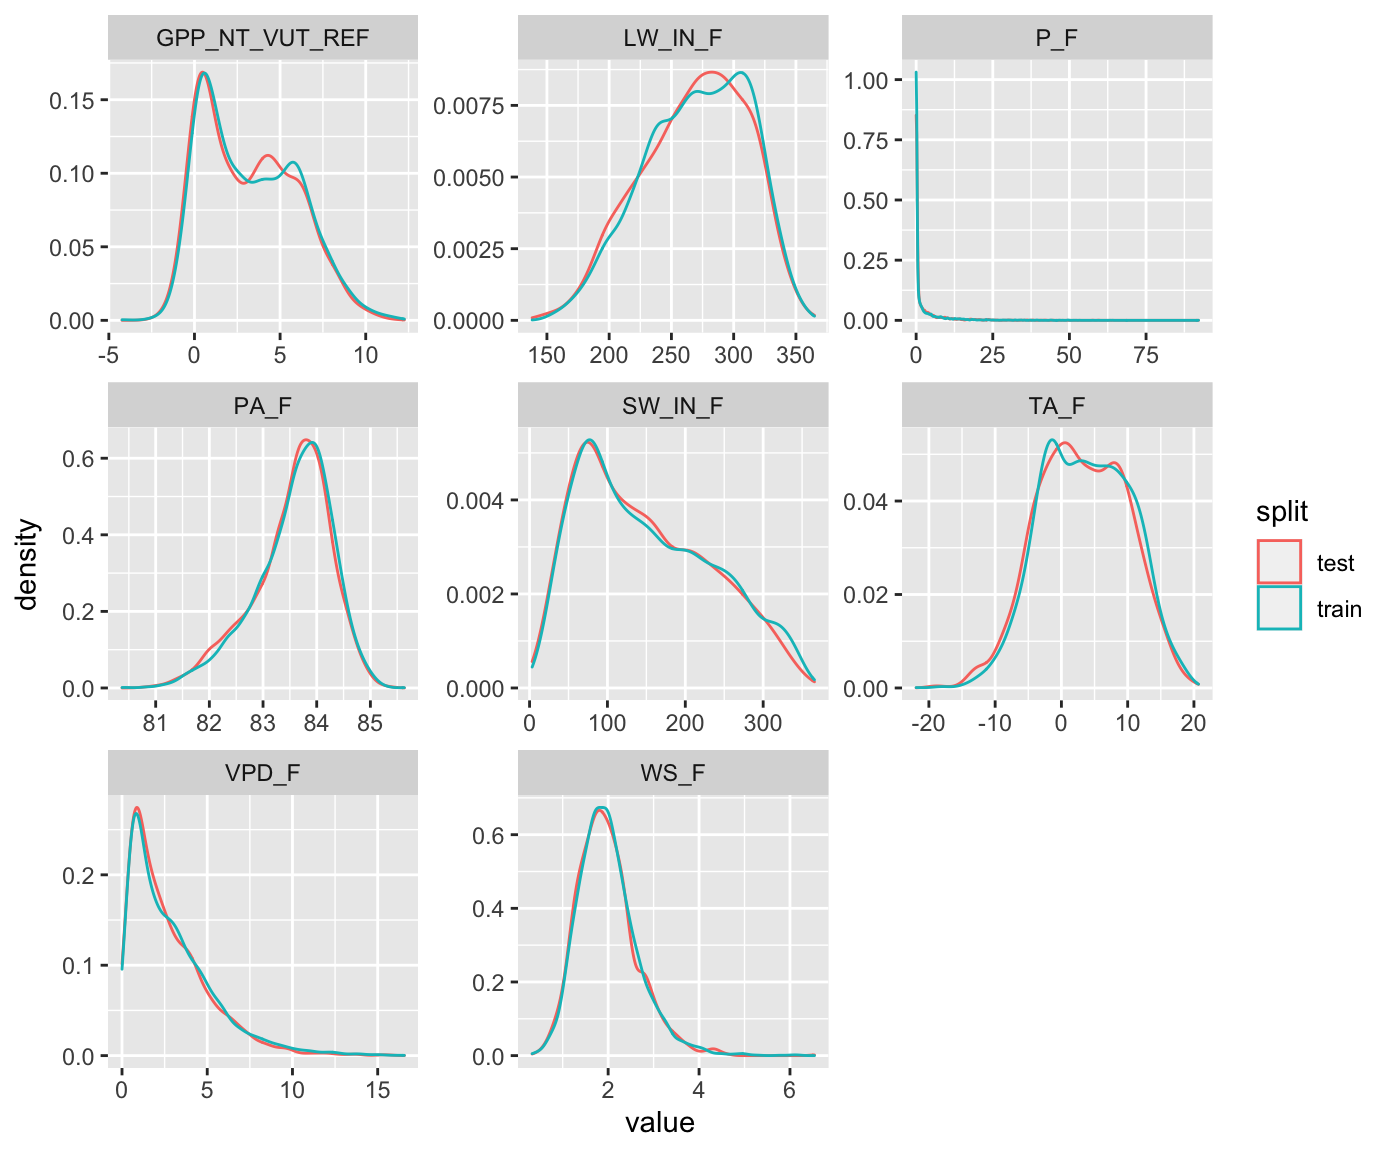
\includegraphics{ml4ec_workshop_files/figure-latex/unnamed-chunk-44-1} \end{center}

The variable \texttt{PA\_F} looks weird and was not significant in the linear model. Therefore, we won't use it for the models below.

\hypertarget{training-5}{%
\subsection{Training}\label{training-5}}

Fit two KNN models on \texttt{ddf\_train} (excluding \texttt{"PA\_F"}), one with \(k = 2\) and one with \(k = 30\), both without resampling. Use the RMSE as the loss function. Center and scale data as part of the pre-processing and model formulation specification using the function \texttt{recipe()}.

\begin{Shaded}
\begin{Highlighting}[]
\FunctionTok{library}\NormalTok{(recipes)}

\DocumentationTok{\#\# model formulation and preprocessing specification}
\NormalTok{myrecipe }\OtherTok{\textless{}{-}} \FunctionTok{recipe}\NormalTok{(}
\NormalTok{  GPP\_NT\_VUT\_REF }\SpecialCharTok{\textasciitilde{}}\NormalTok{ TA\_F }\SpecialCharTok{+}\NormalTok{ SW\_IN\_F }\SpecialCharTok{+}\NormalTok{ LW\_IN\_F }\SpecialCharTok{+}\NormalTok{ VPD\_F }\SpecialCharTok{+}\NormalTok{ P\_F }\SpecialCharTok{+}\NormalTok{ WS\_F, }
  \AttributeTok{data =}\NormalTok{ ddf\_train }\SpecialCharTok{\%\textgreater{}\%} \FunctionTok{drop\_na}\NormalTok{()) }\SpecialCharTok{\%\textgreater{}\%} 
  \FunctionTok{step\_center}\NormalTok{(}\FunctionTok{all\_numeric}\NormalTok{(), }\SpecialCharTok{{-}}\FunctionTok{all\_outcomes}\NormalTok{()) }\SpecialCharTok{\%\textgreater{}\%}
  \FunctionTok{step\_scale}\NormalTok{(}\FunctionTok{all\_numeric}\NormalTok{(), }\SpecialCharTok{{-}}\FunctionTok{all\_outcomes}\NormalTok{())}

\DocumentationTok{\#\# fit model with k=2}
\NormalTok{mod\_knn\_k2 }\OtherTok{\textless{}{-}} \FunctionTok{train}\NormalTok{(}
\NormalTok{  myrecipe, }
  \AttributeTok{data =}\NormalTok{ ddf\_train }\SpecialCharTok{\%\textgreater{}\%} 
    \FunctionTok{drop\_na}\NormalTok{(), }
  \AttributeTok{method =} \StringTok{"knn"}\NormalTok{,}
  \AttributeTok{trControl =} \FunctionTok{trainControl}\NormalTok{(}\StringTok{"none"}\NormalTok{),}
  \AttributeTok{tuneGrid =} \FunctionTok{data.frame}\NormalTok{(}\AttributeTok{k =} \FunctionTok{c}\NormalTok{(}\DecValTok{2}\NormalTok{)),}
  \AttributeTok{metric =} \StringTok{"RMSE"}
\NormalTok{  )}

\DocumentationTok{\#\# fit model with k=30}
\NormalTok{mod\_knn\_k30 }\OtherTok{\textless{}{-}} \FunctionTok{train}\NormalTok{(}
\NormalTok{  myrecipe, }
  \AttributeTok{data =}\NormalTok{ ddf\_train }\SpecialCharTok{\%\textgreater{}\%} 
    \FunctionTok{drop\_na}\NormalTok{(), }
  \AttributeTok{method =} \StringTok{"knn"}\NormalTok{,}
  \AttributeTok{trControl =} \FunctionTok{trainControl}\NormalTok{(}\StringTok{"none"}\NormalTok{),}
  \AttributeTok{tuneGrid =} \FunctionTok{data.frame}\NormalTok{(}\AttributeTok{k =} \FunctionTok{c}\NormalTok{(}\DecValTok{30}\NormalTok{)),}
  \AttributeTok{metric =} \StringTok{"RMSE"}
\NormalTok{  )}
\end{Highlighting}
\end{Shaded}

\hypertarget{prediction-4}{%
\subsection{Prediction}\label{prediction-4}}

With the two models fitted above, predict \texttt{"GPP\_NT\_VUT\_REF"} for both and training and the testing sets, and evaluate them as above (metrics and visualisation).

Which model do you expect to perform better better on the training set and which to perform better on the testing set? Why?

\begin{Shaded}
\begin{Highlighting}[]
\DocumentationTok{\#\# with k = 2}
\FunctionTok{eval\_model}\NormalTok{(}
\NormalTok{  mod\_knn\_k2, }
  \AttributeTok{df\_train =}\NormalTok{ ddf\_train, }
  \AttributeTok{df\_test =}\NormalTok{ ddf\_test}
\NormalTok{  )}
\end{Highlighting}
\end{Shaded}

\begin{center}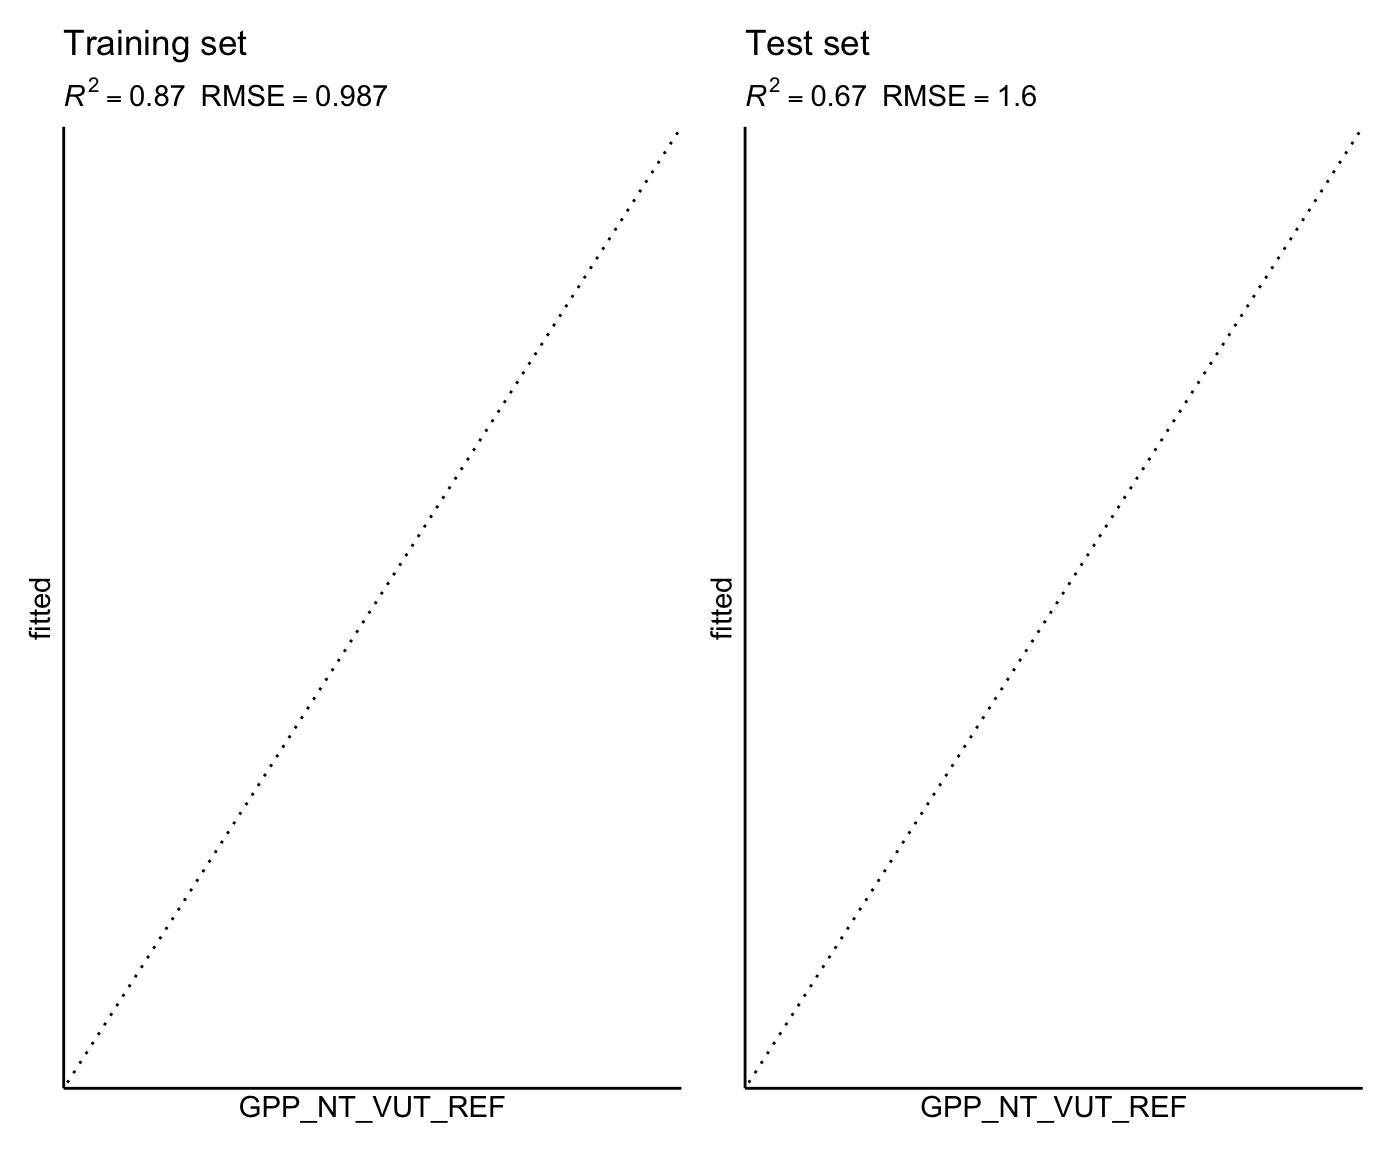
\includegraphics{ml4ec_workshop_files/figure-latex/unnamed-chunk-46-1} \end{center}

\begin{Shaded}
\begin{Highlighting}[]
\DocumentationTok{\#\# with k = 30}
\FunctionTok{eval\_model}\NormalTok{(}
\NormalTok{  mod\_knn\_k30, }
  \AttributeTok{df\_train =}\NormalTok{ ddf\_train, }
  \AttributeTok{df\_test =}\NormalTok{ ddf\_test}
\NormalTok{  )}
\end{Highlighting}
\end{Shaded}

\begin{center}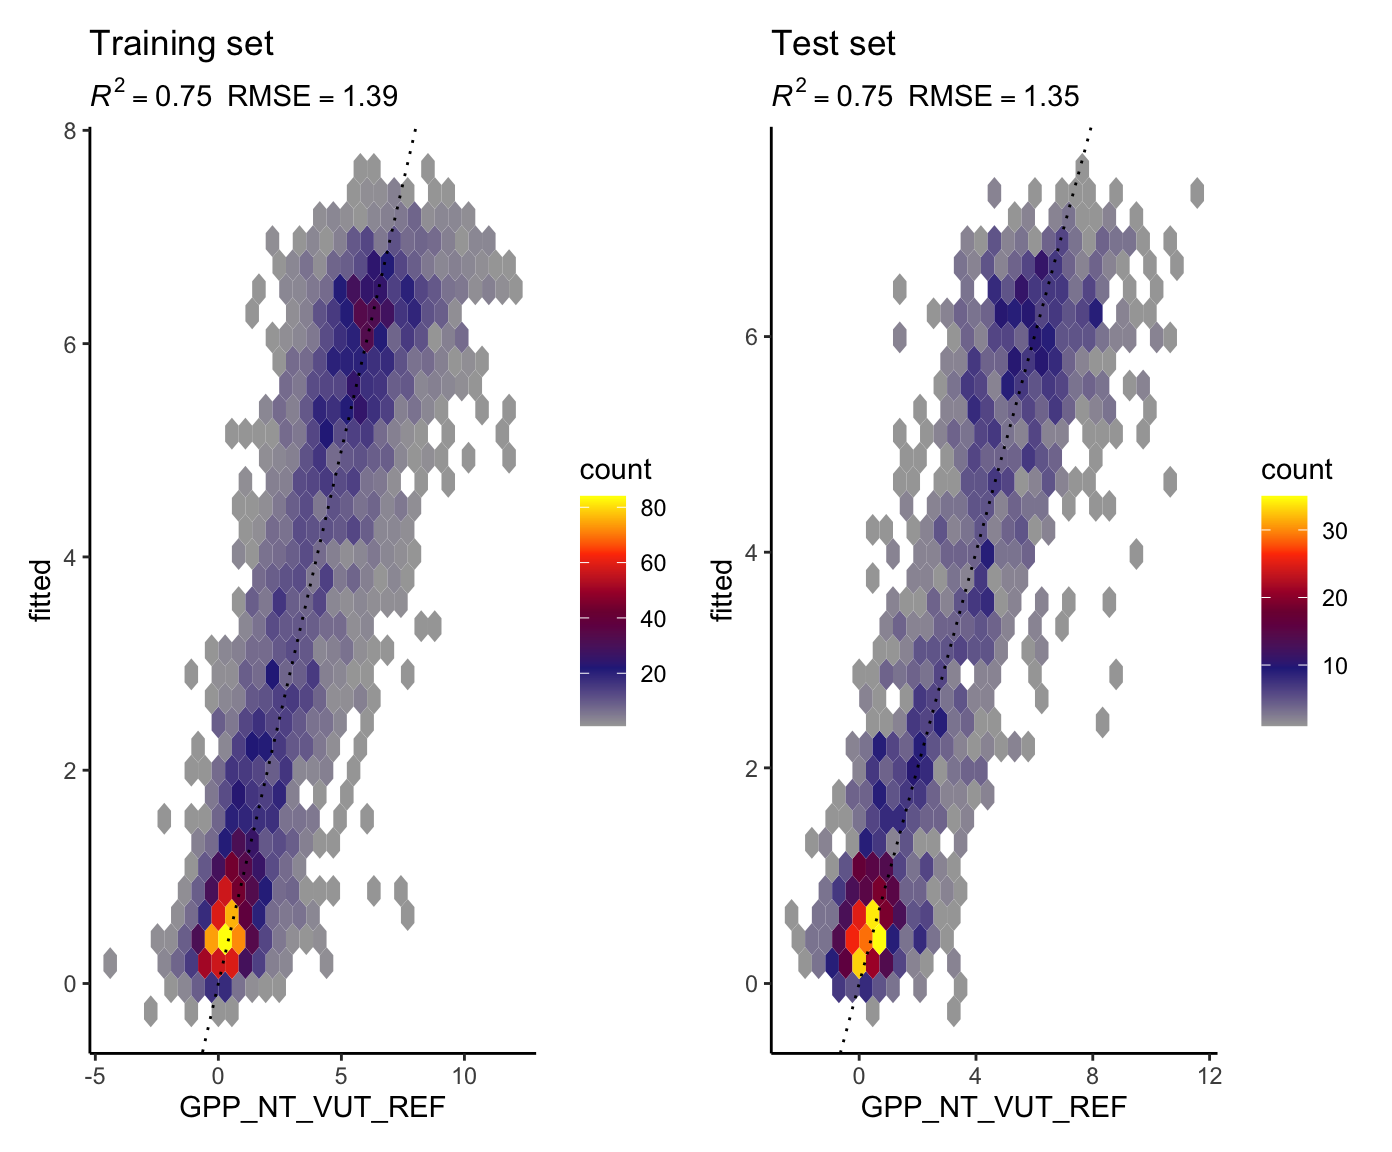
\includegraphics{ml4ec_workshop_files/figure-latex/unnamed-chunk-46-2} \end{center}

\hypertarget{sample-hyperparameters-1}{%
\subsection{Sample hyperparameters}\label{sample-hyperparameters-1}}

Train a KNN model with hyperparameter (\(k\)) tuned, and with five-fold cross validation, using the training set. As the loss function, use RMSE. Sample the following values for \(k\): 2, 5, 10, 15, 18, 20, 22, 24, 26, 30, 35, 40, 60, 100. Visualise the RMSE as a function of \(k\).

Hint:

\begin{itemize}
\tightlist
\item
  The visualisation of cross-validation results can be visualised with the \texttt{plot(model\_object)} of \texttt{ggplot(model\_object)}.
\end{itemize}

\begin{Shaded}
\begin{Highlighting}[]
\NormalTok{mod\_knn }\OtherTok{\textless{}{-}} \FunctionTok{train}\NormalTok{(}
\NormalTok{  myrecipe, }
  \AttributeTok{data =}\NormalTok{ ddf\_train }\SpecialCharTok{\%\textgreater{}\%} 
    \FunctionTok{drop\_na}\NormalTok{(), }
  \AttributeTok{method =} \StringTok{"knn"}\NormalTok{,}
  \AttributeTok{trControl =} \FunctionTok{trainControl}\NormalTok{(}\AttributeTok{method =} \StringTok{"cv"}\NormalTok{, }\AttributeTok{number =} \DecValTok{5}\NormalTok{),}
  \AttributeTok{tuneGrid =} \FunctionTok{data.frame}\NormalTok{(}\AttributeTok{k =} \FunctionTok{c}\NormalTok{(}\DecValTok{2}\NormalTok{, }\DecValTok{5}\NormalTok{, }\DecValTok{10}\NormalTok{, }\DecValTok{15}\NormalTok{, }\DecValTok{18}\NormalTok{, }\DecValTok{20}\NormalTok{, }\DecValTok{22}\NormalTok{, }\DecValTok{24}\NormalTok{, }\DecValTok{26}\NormalTok{, }\DecValTok{30}\NormalTok{, }\DecValTok{35}\NormalTok{, }\DecValTok{40}\NormalTok{, }\DecValTok{60}\NormalTok{, }\DecValTok{100}\NormalTok{)),}
  \AttributeTok{metric =} \StringTok{"RMSE"}
\NormalTok{  )}
\FunctionTok{ggplot}\NormalTok{(mod\_knn)}
\end{Highlighting}
\end{Shaded}

\begin{center}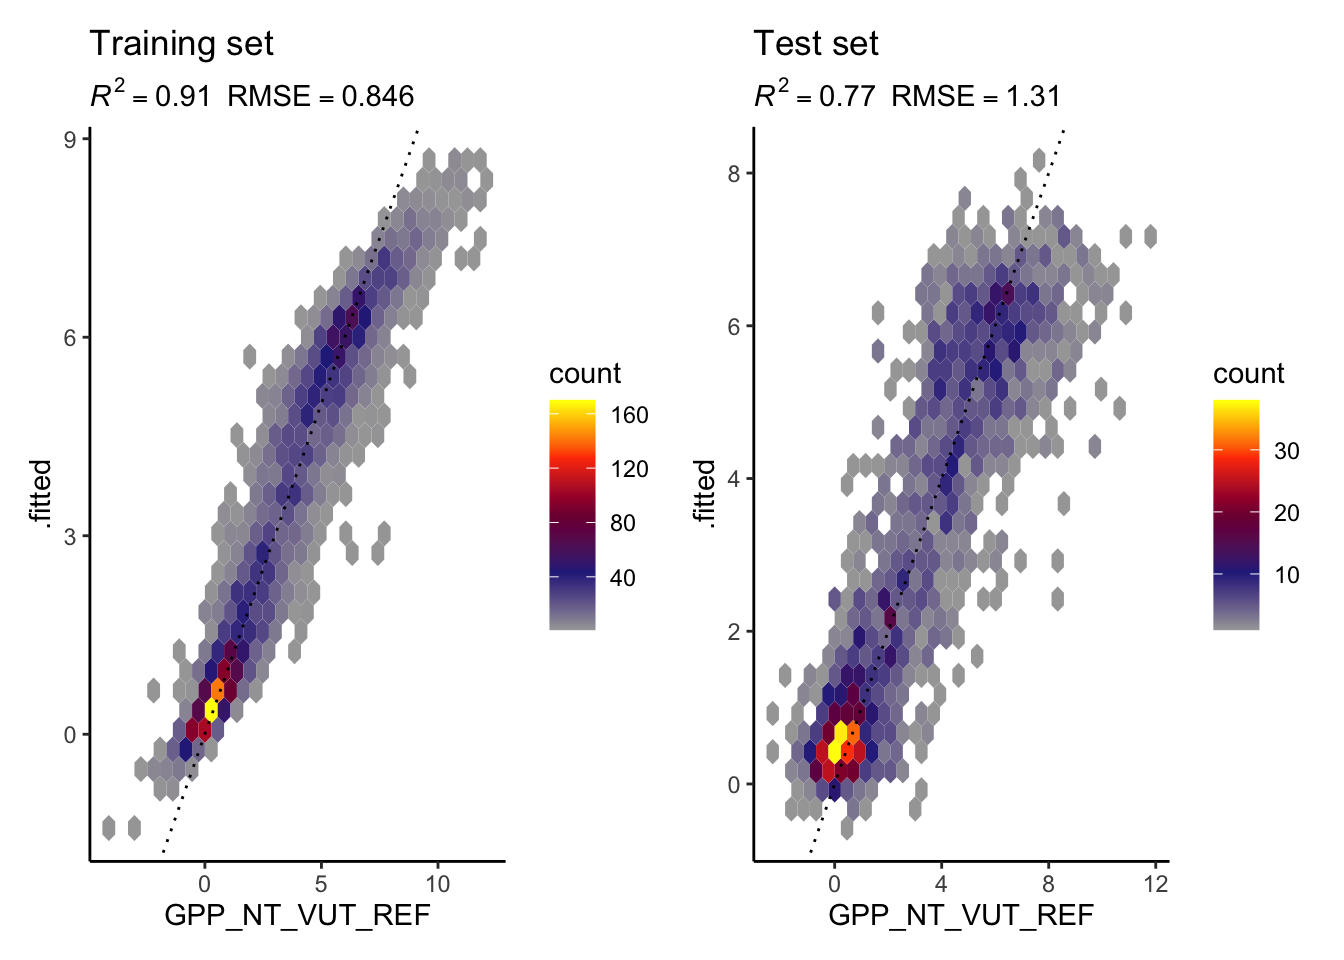
\includegraphics{ml4ec_workshop_files/figure-latex/unnamed-chunk-47-1} \end{center}

\hypertarget{random-forest-2}{%
\section{Random forest}\label{random-forest-2}}

\hypertarget{training-6}{%
\subsection{Training}\label{training-6}}

Fit a random forest model with \texttt{ddf\_train} and all predictors excluding \texttt{"PA\_F"} and five-fold cross validation. Use RMSE as the loss function.

Hints:

\begin{itemize}
\tightlist
\item
  Use the package \emph{ranger} which implements the random forest algorithm.
\item
  See \href{https://topepo.github.io/caret/available-models.html}{here} for information about hyperparameters available for tuning with caret.
\item
  Set the argument \texttt{savePredictions\ =\ "final"} of function \texttt{trainControl()}.
\end{itemize}

\begin{Shaded}
\begin{Highlighting}[]
\FunctionTok{library}\NormalTok{(ranger)}

\DocumentationTok{\#\# no pre{-}processing necessary}
\NormalTok{myrecipe }\OtherTok{\textless{}{-}} \FunctionTok{recipe}\NormalTok{(}
\NormalTok{  GPP\_NT\_VUT\_REF }\SpecialCharTok{\textasciitilde{}}\NormalTok{ TA\_F }\SpecialCharTok{+}\NormalTok{ SW\_IN\_F }\SpecialCharTok{+}\NormalTok{ LW\_IN\_F }\SpecialCharTok{+}\NormalTok{ VPD\_F }\SpecialCharTok{+}\NormalTok{ P\_F }\SpecialCharTok{+}\NormalTok{ WS\_F, }
  \AttributeTok{data =}\NormalTok{ ddf\_train }\SpecialCharTok{\%\textgreater{}\%} 
    \FunctionTok{drop\_na}\NormalTok{())}

\NormalTok{rf }\OtherTok{\textless{}{-}} \FunctionTok{train}\NormalTok{(}
\NormalTok{  myrecipe, }
  \AttributeTok{data =}\NormalTok{ ddf\_train }\SpecialCharTok{\%\textgreater{}\%} 
    \FunctionTok{drop\_na}\NormalTok{(), }
  \AttributeTok{method =} \StringTok{"ranger"}\NormalTok{,}
  \AttributeTok{trControl =} \FunctionTok{trainControl}\NormalTok{(}\AttributeTok{method =} \StringTok{"cv"}\NormalTok{, }\AttributeTok{number =} \DecValTok{5}\NormalTok{, }\AttributeTok{savePredictions =} \StringTok{"final"}\NormalTok{),}
  \AttributeTok{tuneGrid =} \FunctionTok{expand.grid}\NormalTok{( }\AttributeTok{.mtry =} \FunctionTok{floor}\NormalTok{(}\DecValTok{6} \SpecialCharTok{/} \DecValTok{3}\NormalTok{),}
                          \AttributeTok{.min.node.size =} \DecValTok{5}\NormalTok{,}
                          \AttributeTok{.splitrule =} \StringTok{"variance"}\NormalTok{),}
  \AttributeTok{metric =} \StringTok{"RMSE"}\NormalTok{,}
  \AttributeTok{replace =} \ConstantTok{FALSE}\NormalTok{,}
  \AttributeTok{sample.fraction =} \FloatTok{0.5}\NormalTok{,}
  \AttributeTok{num.trees =} \DecValTok{2000}\NormalTok{,          }\CommentTok{\# high number ok since no hperparam tuning}
  \AttributeTok{seed =} \DecValTok{1982}                \CommentTok{\# for reproducibility}
\NormalTok{)}
\NormalTok{rf}
\end{Highlighting}
\end{Shaded}

\begin{verbatim}
## Random Forest 
## 
## 4143 samples
##    8 predictor
## 
## Recipe steps:  
## Resampling: Cross-Validated (5 fold) 
## Summary of sample sizes: 3313, 3315, 3315, 3314, 3315 
## Resampling results:
## 
##   RMSE      Rsquared  MAE     
##   1.401107  0.746519  1.056488
## 
## Tuning parameter 'mtry' was held constant at a value of 2
## Tuning
##  parameter 'splitrule' was held constant at a value of variance
## 
## Tuning parameter 'min.node.size' was held constant at a value of 5
\end{verbatim}

\hypertarget{prediction-5}{%
\subsection{Prediction}\label{prediction-5}}

Evaluate the trained model on the training and on the test set, giving metrics and a visualisation as above.

How are differences in performance to be interpreted? Compare the performances of linear regression, KNN, and random forest, considering the evaluation on the test set.

\begin{Shaded}
\begin{Highlighting}[]
\FunctionTok{eval\_model}\NormalTok{(rf, }\AttributeTok{df\_train =}\NormalTok{ ddf\_train, }\AttributeTok{df\_test =}\NormalTok{ ddf\_test)}
\end{Highlighting}
\end{Shaded}

\begin{center}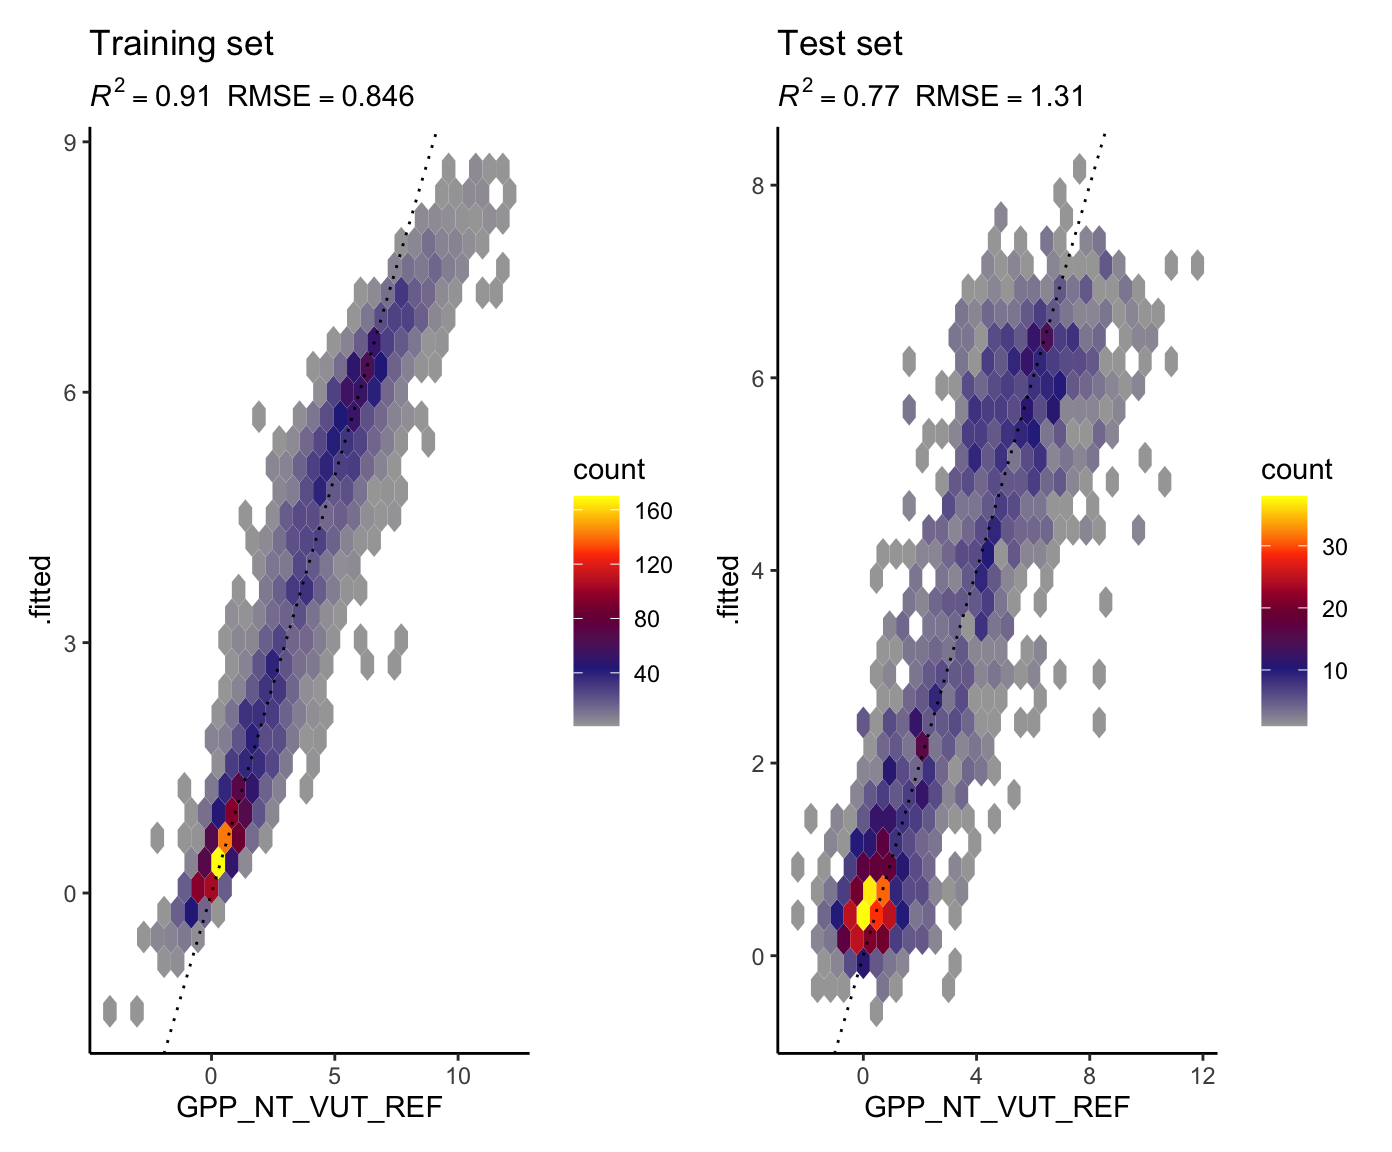
\includegraphics{ml4ec_workshop_files/figure-latex/unnamed-chunk-49-1} \end{center}

Show the model performance (metrics and visualisation) on the validation sets all cross validation folds combined.

Do you expect it to be more similar to the model performance on the training set or the testing set in the evaluation above? Why?

\begin{Shaded}
\begin{Highlighting}[]
\NormalTok{metrics\_train }\OtherTok{\textless{}{-}}\NormalTok{ rf}\SpecialCharTok{$}\NormalTok{pred }\SpecialCharTok{\%\textgreater{}\%} 
\NormalTok{  yardstick}\SpecialCharTok{::}\FunctionTok{metrics}\NormalTok{(obs, pred)}

\NormalTok{rmse\_train }\OtherTok{\textless{}{-}}\NormalTok{ metrics\_train }\SpecialCharTok{\%\textgreater{}\%} 
  \FunctionTok{filter}\NormalTok{(.metric }\SpecialCharTok{==} \StringTok{"rmse"}\NormalTok{) }\SpecialCharTok{\%\textgreater{}\%} 
  \FunctionTok{pull}\NormalTok{(.estimate)}
\NormalTok{rsq\_train }\OtherTok{\textless{}{-}}\NormalTok{ metrics\_train }\SpecialCharTok{\%\textgreater{}\%} 
  \FunctionTok{filter}\NormalTok{(.metric }\SpecialCharTok{==} \StringTok{"rsq"}\NormalTok{) }\SpecialCharTok{\%\textgreater{}\%} 
  \FunctionTok{pull}\NormalTok{(.estimate)}

\NormalTok{rf}\SpecialCharTok{$}\NormalTok{pred }\SpecialCharTok{\%\textgreater{}\%} 
  \FunctionTok{ggplot}\NormalTok{(}\FunctionTok{aes}\NormalTok{(obs, pred)) }\SpecialCharTok{+}
  \FunctionTok{geom\_hex}\NormalTok{() }\SpecialCharTok{+}
  \FunctionTok{scale\_fill\_gradientn}\NormalTok{(}
    \AttributeTok{colours =} \FunctionTok{colorRampPalette}\NormalTok{( }\FunctionTok{c}\NormalTok{(}\StringTok{"gray65"}\NormalTok{, }\StringTok{"navy"}\NormalTok{, }\StringTok{"red"}\NormalTok{, }\StringTok{"yellow"}\NormalTok{))(}\DecValTok{5}\NormalTok{)) }\SpecialCharTok{+}
  \FunctionTok{geom\_abline}\NormalTok{(}\AttributeTok{slope =} \DecValTok{1}\NormalTok{, }\AttributeTok{intercept =} \DecValTok{0}\NormalTok{, }\AttributeTok{linetype =} \StringTok{"dotted"}\NormalTok{) }\SpecialCharTok{+}
  \FunctionTok{labs}\NormalTok{(}\AttributeTok{subtitle =} \FunctionTok{bquote}\NormalTok{( }\FunctionTok{italic}\NormalTok{(R)}\SpecialCharTok{\^{}}\DecValTok{2} \SpecialCharTok{==}\NormalTok{ .(}\FunctionTok{format}\NormalTok{(rsq\_train, }\AttributeTok{digits =} \DecValTok{2}\NormalTok{)) }\SpecialCharTok{\textasciitilde{}}\ErrorTok{\textasciitilde{}}
\NormalTok{                          RMSE }\SpecialCharTok{==}\NormalTok{ .(}\FunctionTok{format}\NormalTok{(rmse\_train, }\AttributeTok{digits =} \DecValTok{3}\NormalTok{))),}
       \AttributeTok{title =} \StringTok{"Validation folds in training set"}\NormalTok{) }\SpecialCharTok{+}
  \FunctionTok{theme\_classic}\NormalTok{()}
\end{Highlighting}
\end{Shaded}

\begin{center}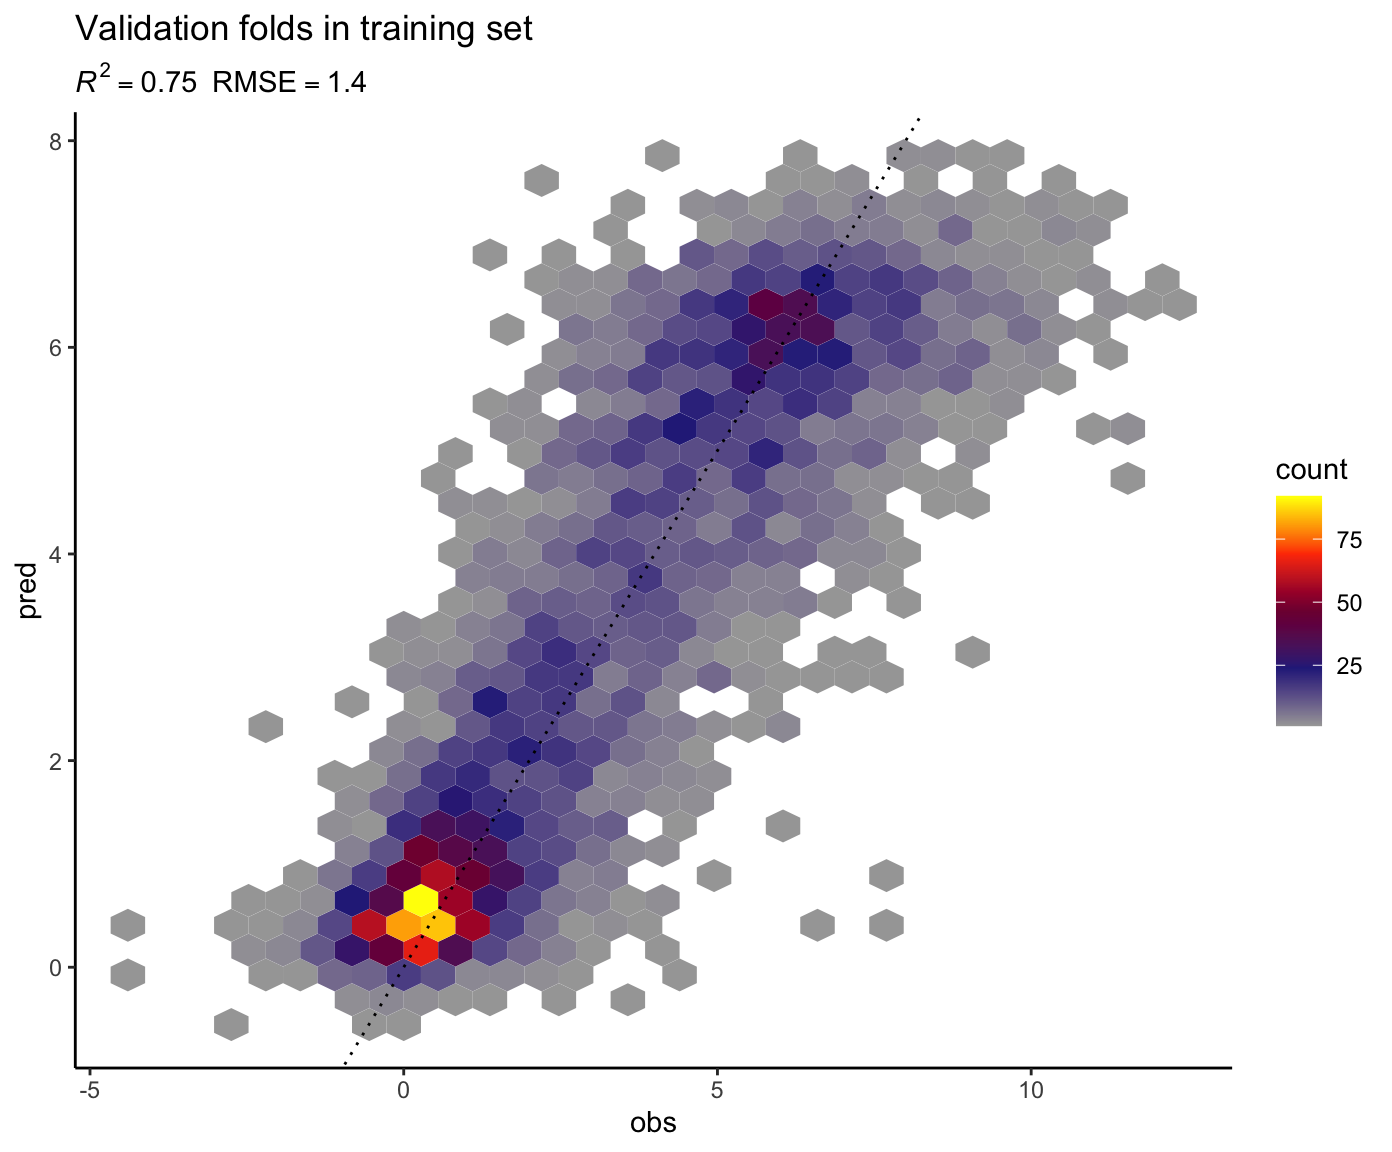
\includegraphics{ml4ec_workshop_files/figure-latex/unnamed-chunk-50-1} \end{center}

  \bibliography{book.bib,packages.bib}

\end{document}
